\documentclass[a4paper,12pt]{thesis}

\usepackage[utf8]{inputenc}

\usepackage{blindtext}


\usepackage[onehalfspacing]{setspace}

\usepackage{adjustbox}
\usepackage[ngerman]{babel}
\usepackage[T1]{fontenc}
\usepackage{amsfonts}
\usepackage{amsmath}
\usepackage{mathtools} 
\usepackage{mathabx}
\usepackage{graphicx}
\usepackage[table]{xcolor}
\usepackage{longtable}
%\usepackage{hyperref}

\usepackage{setspace}

\usepackage{color}
\usepackage{transparent}

\usepackage{tikz}
\usetikzlibrary{positioning}
\usetikzlibrary{arrows,calc}
%\usepackage{pgfplots} % LaTeX
\usepackage{colortbl}
%\usepackage{pgfplotstable}
\usepackage{booktabs, colortbl}

\usepackage{eurosym}

\usepackage{csvsimple}

\usepackage[authoryear]{natbib}
%\bibliographystyle{apalike}
\usepackage[hidelinks]{hyperref}
\bibliographystyle{apalike}

\newcommand*{\captionsource}[2]{%
	\caption[{#1}]{%
		#1%
		\\\hspace{\linewidth}%
		\textbf{Quelle:} #2%
	}%
}

\tikzset{
%Define standard arrow tip
>=stealth',
%Define style for different line styles
help lines/.style={dashed, thick},
axis/.style={<->},
important line/.style={thick},
connection/.style={thick, dotted},
}


\begin{document}

%%% TITELSEITE %%%

\begin{center}								% Beginn einer center-Umgebung. Der Text innerhalb der center-Umgebung wird zentriert. Ansonsten wird Blocksatz verwendet
	\begin{LARGE}								% LARGE beschreibt eine Schriftgröße in Latex. Der Standard ist \normalsize. Eine übersicht der Schriftgrößen steht z.B. auf der Seite: https://www.latex-kurs.de/fragen/schriftgroesse.html 
		Faktoren des Fahrrad Verkehrs in Mannheim						% Text, der nun zentriert und in größerer Schrift geschrieben wird 
	\end{LARGE}								% Die Verwendung der Schriftgröße LARGE wird beendet. Es gilt ab jetzt wieder die normale Schriftgröße.
	
	\vspace{\fill}								% Befehl, der den vertikalen Platz (vspace) "füllt" 
	
	\begin{large}								% Der folgende Text hat nun die Schriftgröße large 
		Maximilian Samuel Weinhold\\					% Durch ein \\ wird eine neue Zeile angefangen. 
		Economics, 6. Semester\\
		505314\\
		mweinhol@uni-muenster.de\\
		
		\vspace{\fill}
		
		Hausarbeit im Rahmen des Seminars zur\\
		Analyse von Fahrrad-Verkehrsdaten\\
		Sommersemester 2021\\
		Institut für Verkehrswissenschaft\\
		Dr. Jan Wessel\\
	\end{large}
	
	\thispagestyle{empty}						% Definiert den Stil für diese Seite. empty bedeutet, dass keine Seitenzahl auf der Seite gedruckt wird. 
	
\end{center}								% Ab nun wird wieder Blocksatz verwendet

\newpage									% Seitenumbruch. Es beginnt eine neue Seite


%\chapter*{Tabellen und Abbildungen}\addchapmark{Tabellen und Abbildungen}
\onehalfspacing	
\thispagestyle{empty}	
\tableofcontents



\begingroup
\let\clearpage\relax
\listoffigures
\listoftables
\endgroup

%\newpage

%\listoffigures

%\newpage


%\listoffigures
%\addcontentsline{toc}{chapter}{Abbildungsverzeichnis}

\chapter{Einleitung}

Die mobile Infrastruktur urbaner Zentren in Deutschland unterliegt einem Wandel, der nicht mehr allein das Ziel einer autofreundlicheren Stadt verfolgt, sondern auch andere Verkehrsteilnehmer hervor hebt. Im Besonderen betrifft diese Entwicklung das Fahrrad. So ist laut \cite{Nobis2019} die Anzahl der Fahrradfahrer innerhalb von 15 Jahren gestiegen sowie die Länge der von ihnen zurückgelegten Wege. Ein Beispiel für diese Entwicklungen ist Mannheim. Denn hier verfolgt die städtische Planung ein 21 Punkte Programm (\cite{Mannheim2010}), dass dazu dienen soll den Anteil des Radverkehrs zu steigern.\\
Im Rahmen dieses Programms installierte die Stadt an verschiedenen Stellen acht Fahrradzähler, deren stündliche Zählungen öffentlich abrufbar sind. Mithilfe dieser Daten lässt sich ein Regressionsmodell entwickeln, dass die kausalen Einflüsse auf den Radverkehr erklärt und das Aufkommen von Fahrrädern vorhersagen kann.\\
Nach einem Überblick über die aktuelle Literatur zu diesem Thema und einer genaueren Beschreibung der verwendeten Daten möchte diese Hausarbeit in zwei Abschnitten ein statistisches Modell entwickeln. Im ersten Abschnitt liegt der Fokus auf die kausalen Zusammenhänge. Im zweiten Teil geht es um die eigene Forschungsfrage: welches Modell kann man wählen, um die Vorhersage Kraft zu maximieren? Im besten Fall ließe sich das Modell extrapolieren, sodass eine Topographie des Fahrradverkehrs absehbar wäre auch an Stellen ohne Zählstationen.\\
Diese Hausarbeit baut vornehmlich auf \cite{Wessel2020} und seine Methodik auf, der primär untersuchte welchen Einfluss Wettervorhersagen und tatsächliches Wetter auf den Radverkehr in verschiedenen deutschen Städten haben.\\
%Darüber hinaus (Wenn Zeit übrig bleibt) wollen wir versuchen die Methoden von \cite{PRATI201744} ebenfalls zu verwenden, um ein Model primär zu Vorhersage des extrapolierten Fahrradaufkommens zu entwickeln.

\chapter{Literaturüberblick}

Da diese Arbeit im Rahmen eines Seminares bei Dr. Jan Wessel entstanden ist, verfolgt sie eine ähnliche Methodik wie bei \cite{Wessel2020}. Dort wird der Frage nachgegangen, wie sehr Wettervorhersagen und tatsächliches Wetter einen Einfluss auf das Aufkommen der Fahrradfahrer hat. Dazu entwickelt er ein Log-lineares Regressionsmodell, das nicht nur die notwendigen Wetterdaten berücksichtigt, sondern auch andere wesentliche Effekte wie Feiertage, Schul- und Semesterferien. Sein Modell kommt zu einem adjusted $R^2$ von 78 \%. Die Daten für das Modell stammen von 188 Zählstationen in ganz Deutschland. Daneben untersuchen auch andere Forscher Fragen zum Thema des Verkehrsaufkommens von Fahrrädern. Z.b. untersuchen \cite{ZHAO2018826} und \cite{Hong2022} den Einfluss von Feinstaubbelastungen auf den Fahrradverkehr. Dabei verwenden diese, ähnlich wie \cite{Wessel2020}, Zeitreihendaten. Aber nicht nur Einflüsse äußerer und zeitlicher Umstände wie Wetter oder Feinstaub sind interessante Variablen. \cite{HANKEY2021102651} gehen im Speziellen auf räumliche Daten ein. Sie beobachten über 4000 Zählstellen in den USA und verwenden Google Streetview Bilder und einen Pixelerkennungsalgorithmus. Ein anderes interessantes Forschungsthema, das in Verbindung zu Fahrraddaten steht, ist die Vorhersage von Verkehrsunfällen, in die Fahrradfahrer verwickelt sind. Diesem Thema gehen \cite{PRATI201744} nach. Sie greifen hierbei nicht auf Regressionsmodelle zurück, sondern auf CHAID (Chi-square Automatic Interaction Detectors) Entscheidungsbäume und auf Bayesian Netzwerkanalysen. Entscheidungsbäume sind für dieses Thema ebenfalls eine interessante Methode. Im Anhang in der Darstellung \ref{DecisionTree} ist ein Entscheidungsbaum, beruhend auf den Datensatz aus Mannheim, dargestellt. Dennoch verwenden wir folgend ausschließlich Regressionsmodelle.

%Hier noch mehr bearbeiten. Vor allem im Bezug auf die eigene Vorschungsfrage.

\chapter{Beschreibung der Daten}

Die Bearbeitung des Modells baut überwiegend auf zwei Datenquellen auf. Am wichtigsten sind die Fahrradzählstationen Mannheims, die öffentlich im Netz zugänglich sind (Link: \url{https://mannheim.opendatasoft.com/page/home/}). Hier sind stündliche Werte gezählter Fahrräder verfügbar an acht verschiedenen Stellen in der Stadt sowie Längen und Breitengrad der Position, Standortname, Zeit und Datum. Zwei dieser Zählstation waren nur in eine Richtung verfügbar (Kurt Schuhmacher und Konrad Adenauer Brücke). Deswegen werden diese der Einfachheit halber mal zwei multipliziert. Im zweiten Schritt werden diese Daten mit stündlichen Daten des Deutschen Wetter Dienstes zur Lufttemperatur in 2 Meter Höhe, zur relativen Feuchte, zum Bedeckungsgrad, zum Niederschlag und zur Sonnenstrahlung verbunden.\\
\cite{ZHAO2018826} und \cite{Hong2022} zeigen, dass auch die Feinstaubbelastung den Radverkehr beeinflussen kann. Grundsätzlich wären die dazu notwendigen Daten aus Mannheim über \url{Opensensemap.org} zugänglich, jedoch nicht für den gesamten Betrachtungszeitraum. Da \cite{ZHAO2018826} und \cite{Hong2022} ihre Forschung in ostasiatischen Ballungsräumen betrieben haben und in einer Stadt wie Mannheim nicht die selbe Feinstaubbelastung zu erwarten ist, kann man von dieser Variable nicht erhoffen, dass sie die notwendige Erklärungskraft bringt, um einen Wegfall des Betrachtungszeitraumes zu rechtfertigen, weshalb Feinstaubmessungen keinen Weg in den Datensatz gefunden haben.\\
Dafür ist es wichtig Feiertage, Schulferien und Semesterferien zu berücksichtigen. Hier könnte potentiell eine geographische Besonderheit Mannheims eine Rolle spielen, denn das Stadtgebiet grenzt direkt zu zwei verschiedenen Bundesländern an. Zum einem liegt auf dem gegenüberliegenden Rheinufer die Stadt Ludwigshafen, die bereits in Rheinland Pfalz liegt. Zwischen beiden Städten herrscht ein reger Verkehr, weshalb anzunehmen ist, dass voneinander abweichende Feiertage in Rheinland Pfalz und Baden Württemberg eine Rolle spielen könnten. Ebenso grenzt Hessen an Mannheim an. Jedoch nicht in einer Reichweite, die für Fahrradfahrer realistisch erscheint und nicht mit einer Stadt, die vergleichbar groß wie Ludwigshafen wäre. Somit finden Feiertage für Hessen keinen Weg ins Model.\\
Dies gilt ebenso für die Schulferien. Es ist anzunehmen, dass innerhalb Mannheims, Schulen überwiegend von Mannheimern besucht werden, weshalb nur die Schulferien von Baden Württemberg im Datensatz zu finden sind. Neben Schülern fahren ebenso häufig Studenten Fahrrad. Die größte Hochschulbildungseinrichtung ist die Universität Mannheim, deren Semesterferien eine signifikante Rolle spielen dürften.

\begin{figure}[!ht]
	\centering
	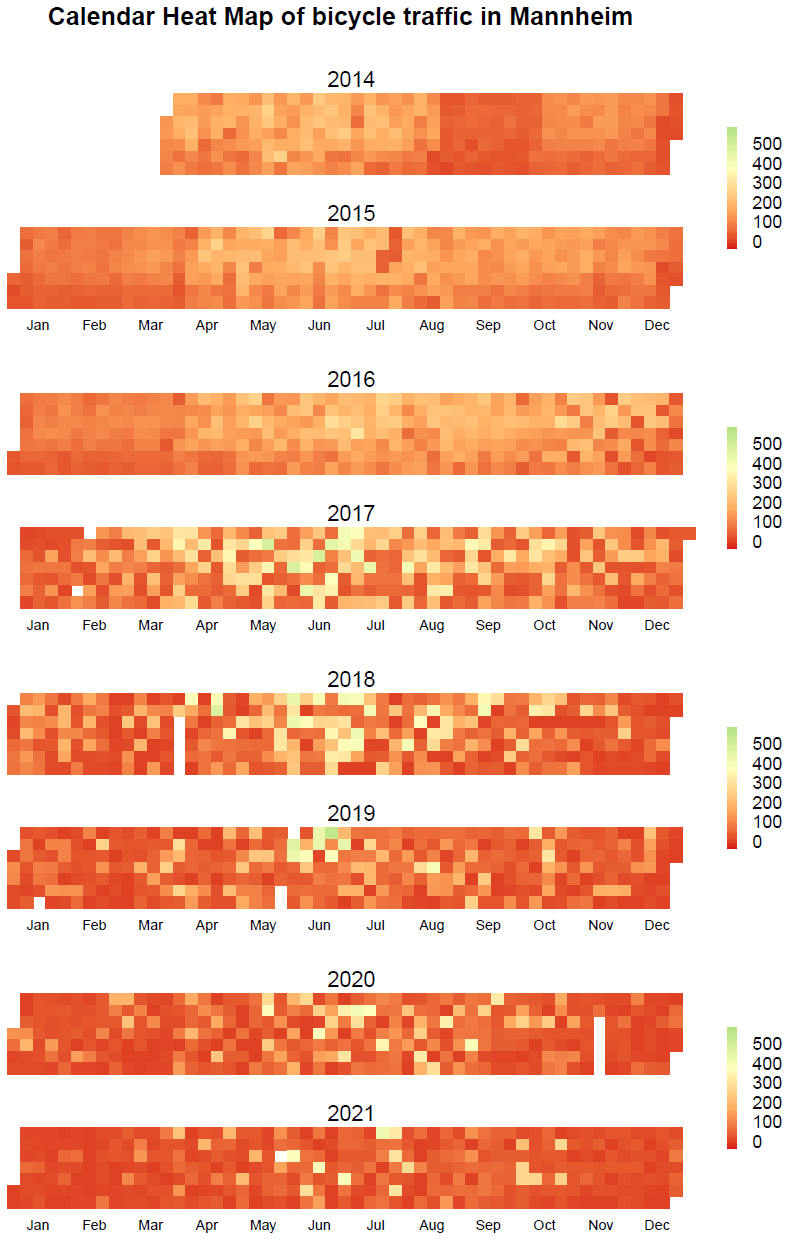
\includegraphics[width=\textwidth]{Plots/CalendarHeatMap.png}
	\caption{Ausprägungen des Fahrradaufkommens}
	\label{fig:calendarheatmap}
\end{figure}

Fügt man all diese Daten zusammen, erhält man einen Datensatz der 410891 Beobachtungen umfasst. Die Ausprägungen pro Tag sind der Darstellung \ref{fig:calendarheatmap} zu entnehmen. Dabei fallen zwei Dinge vornehmlich auf. Zum einem sehen wir, wie gegen Ende 2016 die Varianz der Ausprägungen zu nimmt. Dies hängt mit der Anzahl der Zählstationen zusammen. Die früheste Zählstation an der Renzstraße ging 2014 in Betrieb. Weitere folgten erst 2016. Je mehr Zählstationen mit unterschiedlichen Verkehrsströmen messen, desto höher ist die tägliche Varianz in den Zähldaten. Weiterhin fallen einige wenige weiße Stellen auf. Dies hängt mit unvollständigen Wetterdaten zusammen. Die Menge fehlender Daten fällt hier aber in einen vertretbaren Rahmen, wobei fehlende Tage nicht weiter mit wichtigen Variablen korrelieren.

Einen Überblick über die acht Zählstationen in Mannheim ist in Abbildung \ref{Figure1} zu sehen, wobei zur Erstellung der Graphik ein R Paket genutzt wurde nach \cite{Kahle2013}. Am Farbgradienten ist zu sehen, wie viele Fahrradfahrer pro Stunde die Zählstationen passieren. Zudem ist der Name der Zählstation eingeblendet zudem das Jahr, seitdem diese Station installiert ist.\\
Weitere Variablen wurden aus dem Datum erzeugt. So befindet sich im Datensatz eine binäre Dummy Variable für das Wochenende und eine für Sommermonate. Weiterhin nutzen wir Jahr, Monat, Tag und Stunde als Faktorvariablen, wobei wir nächtliche Stunden zwischen 22 und 5 Uhr ausgeschlossen haben.\\
Zu Abweichungen des Fahrradverkehrs konnte es während der Corona Krise kommen, wo Teile des öffentlichen Lebens still standen und damit auch das Verkehrsaufkommen. Deshalb beinhaltet der Datensatz zwei Variablen, eine Dummy Variable, die vor Ausbruch von Corona null ist und eine Dummy Variable für den Zeitraum der Kontaktbeschränkungen.

\begin{figure}[!ht]
	\centering
	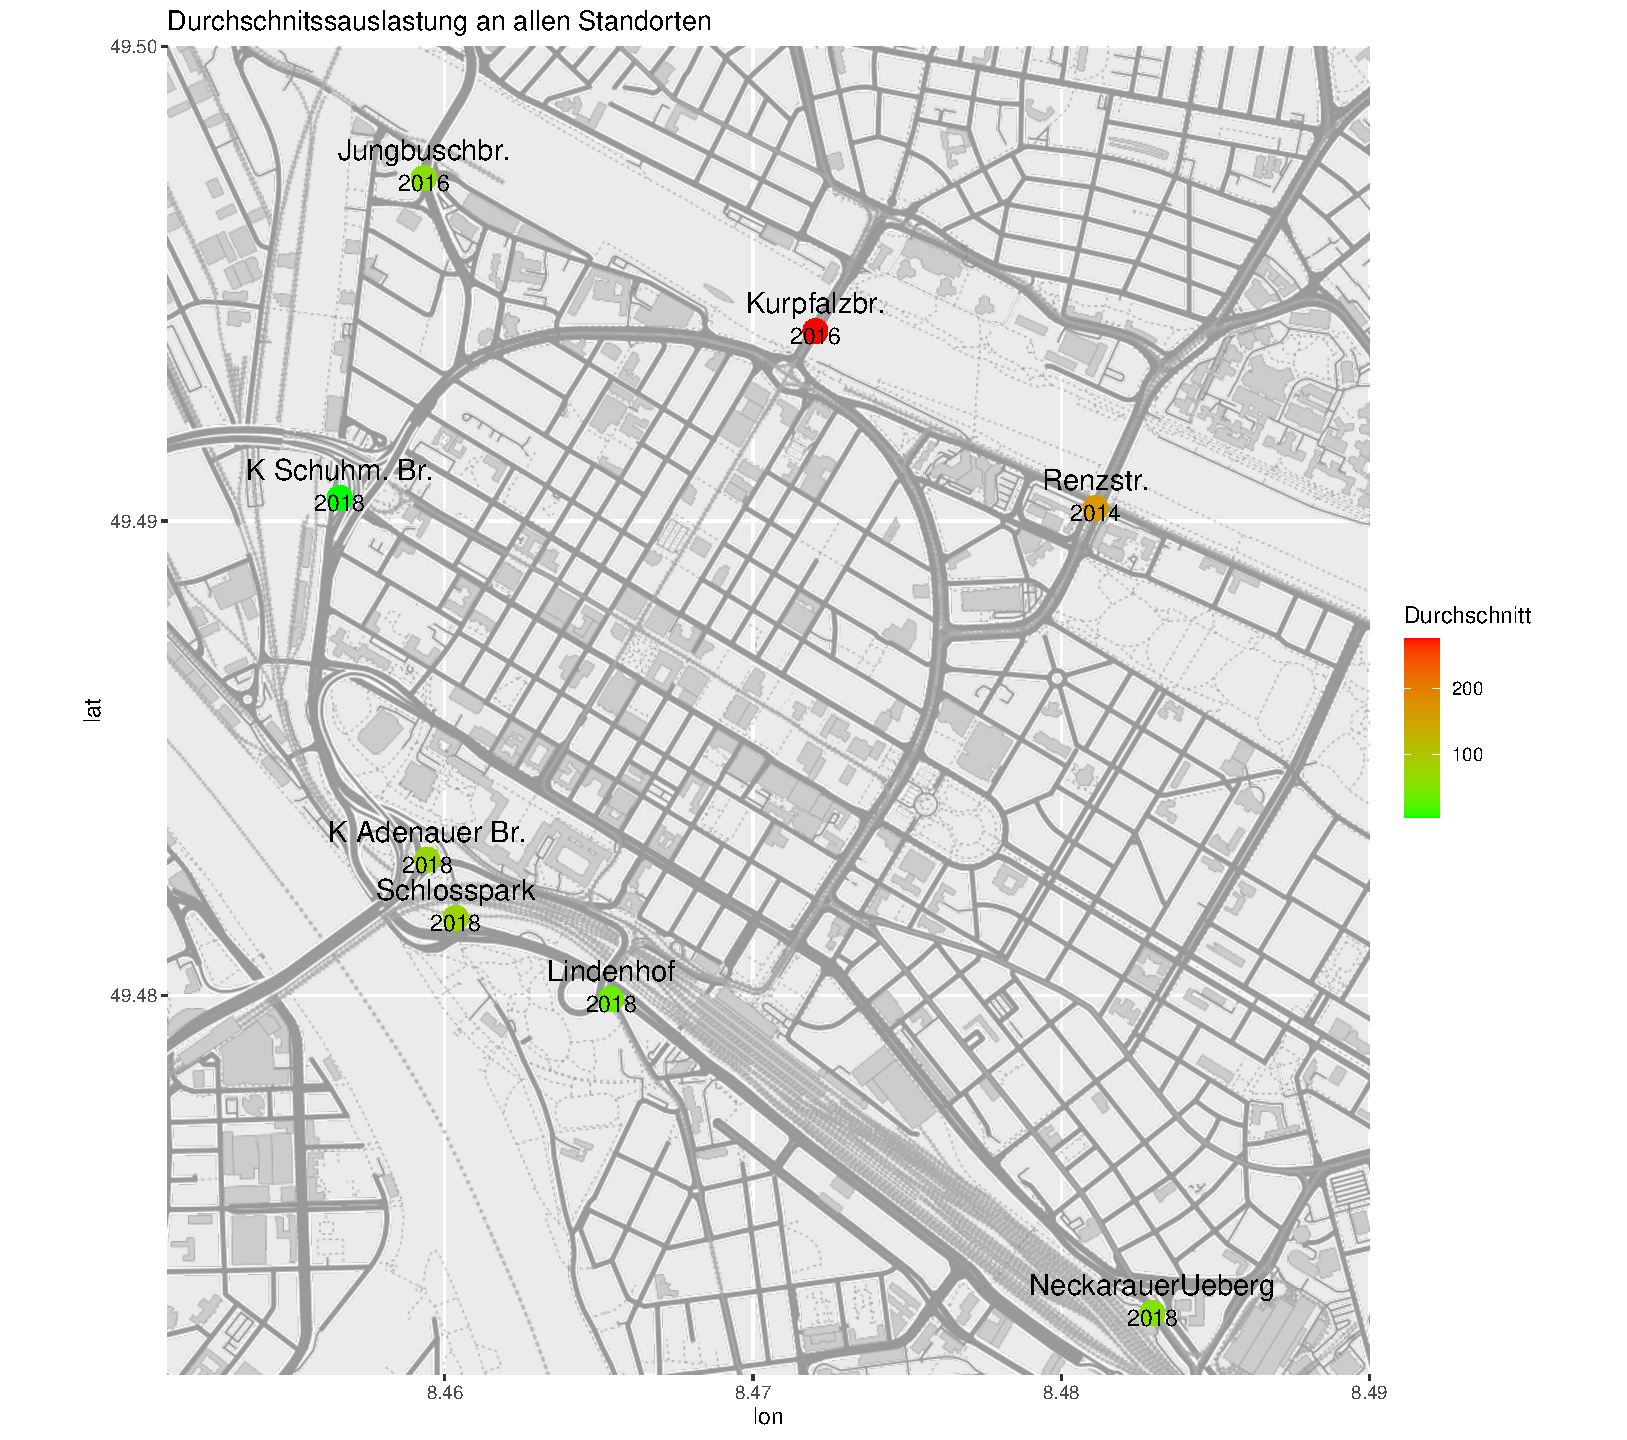
\includegraphics[width=\textwidth]{Plots/Karte_Durchschnittsauslastung.pdf}
	\caption{Zählstationen im Überblick}
	\label{Figure1}
\end{figure}



\begin{figure}[!ht]
	\centering
	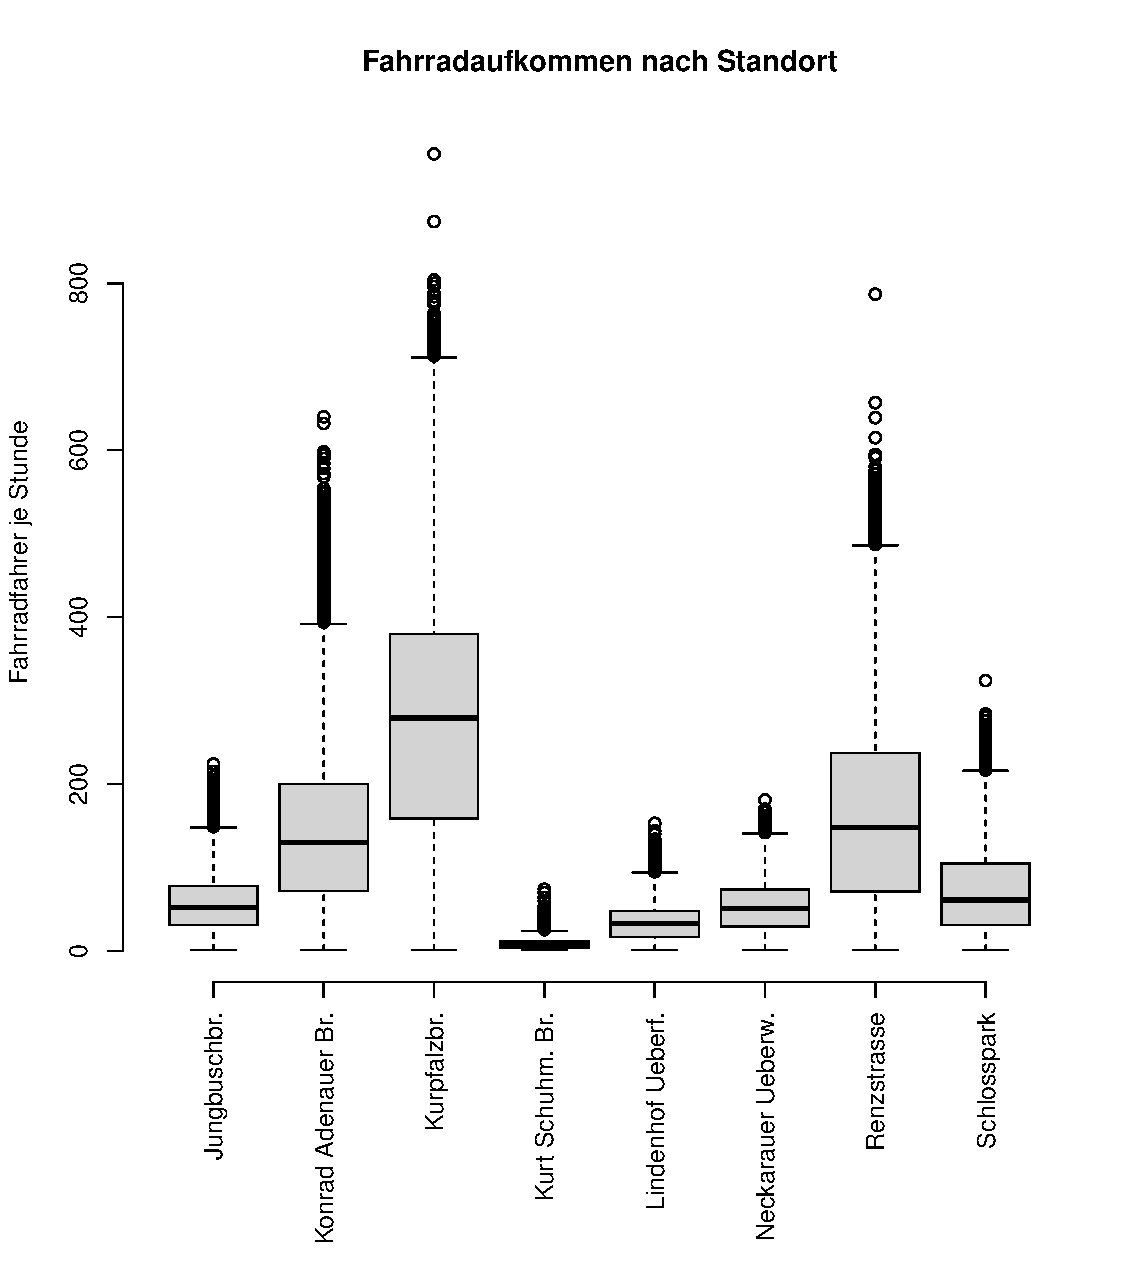
\includegraphics[width=\textwidth]{Plots/Boxplot_Stationen.pdf}
	\caption{Boxplots zu den Zählstationen}
	\label{BoxplotStationen}
\end{figure}

\begin{table}[!ht]
	\centering
	\caption{Datensatz Übersicht}
	\begin{tabular}[t]{rllllll}
		\toprule
		Name & Min & Durchschnitt & Max & Stand.abw. & Korrelation \\ 
		\midrule
		Zählstand & 1 & 116.78 & 955 & 122.74 & 1 \\ 
		Distanz z Uni & 208.36 & 1122.51 & 1875.72 & 583.35 & 0.26 \\ 
		Wochenende & 0 & 0.28 & 1 & 0.45 & -0.21 \\ 
		Sommer & 0 & 0.48 & 1 & 0.5 & 0.15 \\ 
		Feiertag BW & 0 & 0.03 & 1 & 0.18 & -0.09 \\ 
		Feiertag RP & 0 & 0.03 & 1 & 0.18 & -0.08 \\ 
		Schulferien BW & 0 & 0.32 & 1 & 0.47 & 0.04 \\ 
		Semesterferien & 0 & 0.48 & 1 & 0.5 & -0.03 \\ 
		Niederschlag & 0 & 0.07 & 30.4 & 0.49 & -0.03 \\ 
		Temperatur & -13 & 12.67 & 39.4 & 8.33 & 0.24 \\ 
		Wind & 0.1 & 3 & 14.4 & 1.65 & -0.02 \\ 
		Rel. Feuchte & 14 & 69.24 & 100 & 20.3 & -0.23 \\ 
		Sonne & 0 & 19.22 & 60 & 24.82 & 0.17 \\ 
		Bedeckung & 0 & 5.72 & 8 & 3.14 & -0.08 \\ 
		Corona & 0 & 0.42 & 1 & 0.49 & -0.16 \\ 
		Kontaktbeschr & 0 & 0.11 & 1 & 0.32 & -0.09 \\ 
		\hline
	\end{tabular}
	\label{Tabelle1}
\end{table}

\chapter{Deskriptive Analyse}

\section{Regressionsanalyse}

Vorerst sind die gesammelten Daten trotz des Umfangs recht nutzlos, da sie allein wenig Antworten geben. Durchschnitte und Standardabweichungen einzelner Variablen, wie der Temperatur oder des Fahrrad Aufkommens, geben durchaus Aufschluss nie aber in einem größeren Zusammenhang. Doch was eigentlich von Interesse ist was den Fahrradverkehr beeinflusst. Dies mündet z.B. in der Frage welche Rolle der Regenfall beim Fahrradverkehr spielt, oder ob mehr Fahrradfahrer an Feiertagen auf Mannheims Straßen anzufinden sind. Dies muss nicht nur qualitativ, sondern auch quantitativ beantworten.\\
Ein Mittel, um an diese Informationen zu kommen, ist die Regressionsanalyse. Diese versucht den Zusammenhang zu messen, in dem zwei Variablen zu einander stehen. So könnte man z.B. versuchen zu messen, wie sehr sich das Aufkommen an Fahrradfahrer unterscheidet in der Entfernung zur Universität Mannheim. Dargestellt ist dies in der Abbildung \ref{Figure2}. Mithilfe der Regressionsanalyse kann man nun durch diese Punkte an den Positionen der acht Zählstationen jene Linie ziehen, die das Verhältnis mathematisch am besten repräsentiert, indem sie die quadratischen Abstände der Datenpunkte zur Linie selbst minimiert. Natürlich verhält sich nicht alles linear zu einander. Deswegen kann man auch auf quadratische oder kubische Terme zurückgreifen. Und wie man in der Darstellung sieht, beschreibt die kubische Relation scheinbar das Verkehrsaufkommen am besten. Doch ist es zu bezweifeln, dass allein eine Variable zu einer präzisen Vorhersage führt.\\

\begin{figure}[!ht]
	\centering
	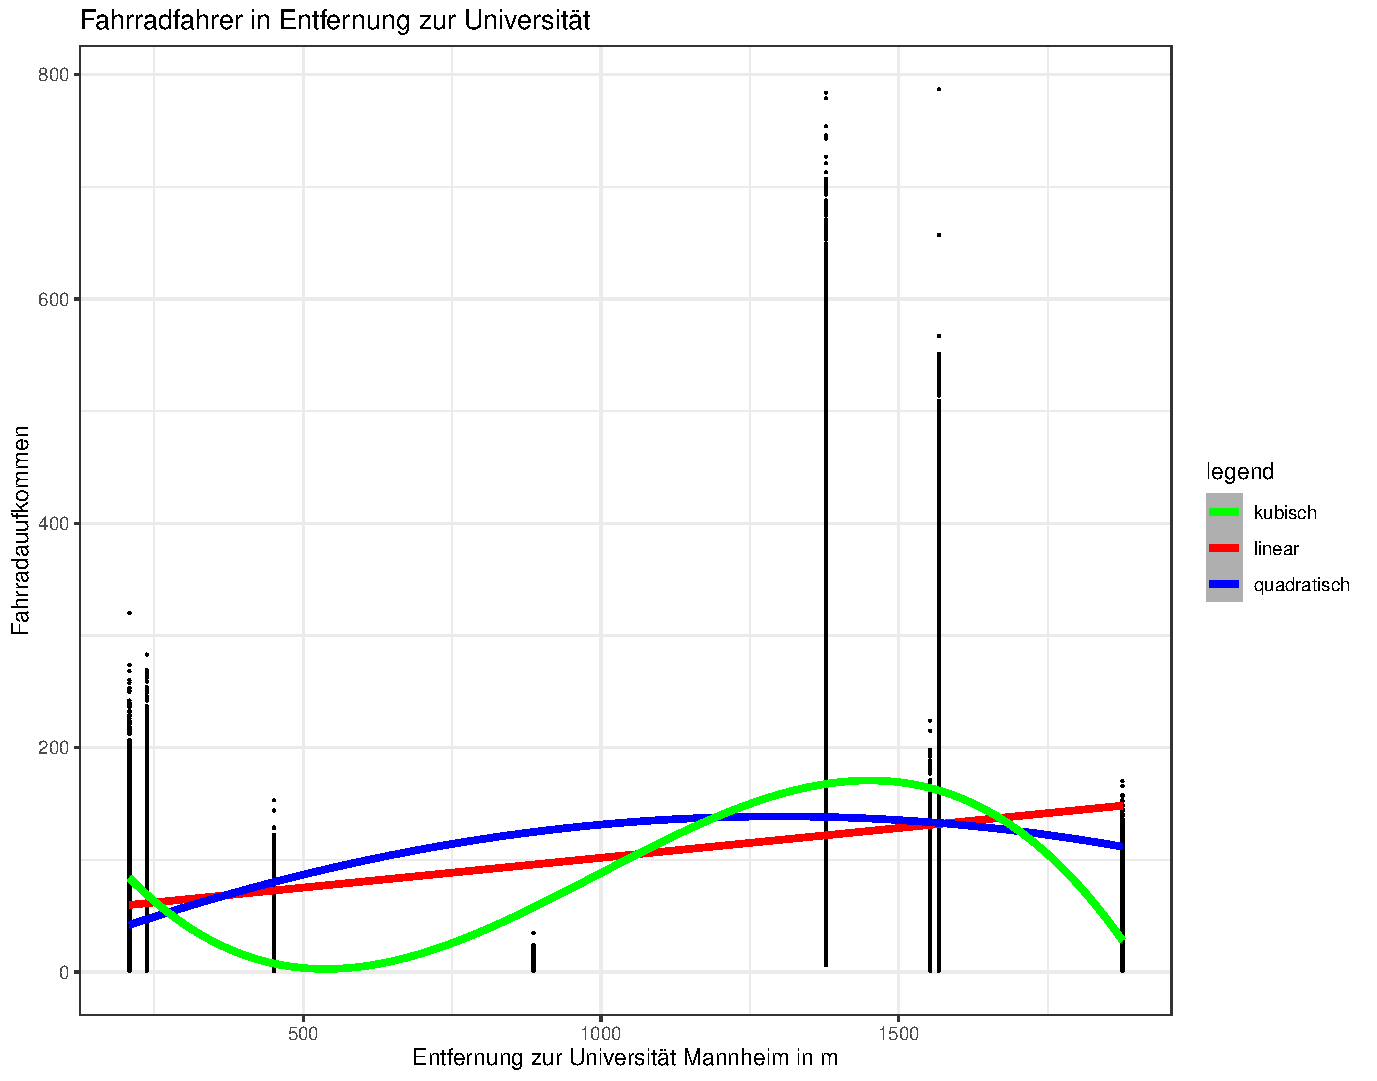
\includegraphics[width=\textwidth]{Plots/Regression_Bsp.pdf}
	\caption{Fahrräder in Entfernung zur Universität Mannheim\\Graphisches Beispiel einer Regression}
	\label{Figure2}
\end{figure}

Nimmt man weitere Variablen in das Regressionsmodell auf, die den Fahrradverkehr erklären könnten, wie z.B. Wetterbeobachtungen oder Ferien- und Feiertage, dann steigt die Genauigkeit (Fit) des Modells. Das heißt wir können präzisere Vorhersagen treffen, weil wir uns ein mehrdimensionales Model schaffen. Dies nennt man dann auch die multiple Regressionsanalyse. Lässt man wiederum wichtige Variablen aus, dann kann das auch die Aussage über die Kausalität verzerren durch den Bias einer ausgelassenen Variable. Deswegen ist es wichtig, die richtigen und sinnigen Variablen in das Model aufzunehmen. Im folgendem Modell sind Wetterdaten und Ferien- Feiertage mit inbegriffen. Zusätzlich verwenden wir eine Dummy Variable für die Sommer Monate und eine Dummy Variable für alle Zeiträume, die von Corona Kontaktbeschränkungen betroffen waren. Nicht direkt dargestellt in der Übersicht \ref{reg1}, sind Dummy Variablen, für die vollen Stunden, Wochentage, Monate und Jahre, sowie für die den Namen der Station als Faktor, damit das Modell zwischen den verschiedenen Leveln der Zählstationen unterscheiden kann, denn der Verkehr an den einzelnen Stationen weicht stark voneinander ab, wie man auch in der Darstellung \ref{BoxplotStationen} sieht.\\

\begin{table}[!ht]
	\centering
	\caption{Log-Lineares Regressionsmodell}
	\begin{tabular}[t]{lc lc lc lc lc lc}
		\toprule
		& Koeffizient & Std Abw & t-Wert & Pr(>|t|) & \\
		\midrule
		%Intercept & -0.184 & (0.015) &\\
		Leichter Nieselregen & -0.186767 & (0.015737) & -11.86798 & 6.8481e-06 & ***\\
		Starker Nieselregen & -0.252077 & (0.011276) & -22.35570 & 9.0628e-08 & ***\\
		Leichter Regen & -0.335288 & (0.020819) & -16.10480 & 8.6516e-07 & ***\\
		Moderater Regen & -0.363761 & (0.019870) & -18.30659 & 3.5941e-07 & ***\\
		Starker Regen & -0.382894 & (0.044853) & -8.53673 & 6.0076e-05 & ***\\
		Heftiger Regen & -0.205909 & (0.052566) & -3.91711 & 5.7704e-03 & **\\
		Temperatur & 0.036746 & (0.004933) & 7.44970 & 1.4326e-04 & ***\\
		Temperatur$^2$ & -0.000496 & (0.000054) & -9.11186 & 3.9361e-05 & ***\\
		Wind & -0.041435 & (0.002633) & -15.73843 & 1.0125e-06 & ***\\
		rel. Feuchte & -0.003825 & (0.001071) & -3.57128 & 9.0814e-03 & **\\
		Sonne & -0.000124 & (0.000082) & -1.51990 & 1.7234e-01 & \\
		Bedeckung & -0.008739 & (0.001070) & -8.16766 & 7.9824e-05 & ***\\
		FeiertagBW & -0.459730 & (0.081119) & -5.66738 & 7.6062e-04 & ***\\
		FeiertagRP & -0.427518 & (0.060086) & -7.11505 & 1.9112e-04 & ***\\
		SchulferienBW & -0.140156 & (0.019901) & -7.04263 & 2.0371e-04 & ***\\
		SemesterferienUM & -0.159926 & (0.030295) & -5.27895 & 1.1494e-03 & **\\
		Sommer & 0.084612 & (0.020959) & 4.03704 & 4.9514e-03 & **\\
		Kontaktbeschr & -0.135452 & (0.026406) & -5.12952 & 1.3544e-03 & **\\
		\midrule
		Num.Obs. & 410891& & RMSE & 0.633826 & \\
		R2 Adj. & 0.785286 &  &  &  & \\
		\bottomrule
		Fixed Effects & Standort & Stunde & Wochentag & Jahr & \\
		Signifikanz: & *p<0.1; & **p<0.05; &***p<0.01 & &\\
	\end{tabular}
\label{reg1}
\end{table}

Interessant sind für uns in der Tabelle \ref{reg1} die Koeffizienten und die Signifikanzniveaus. Wobei wir berücksichtigen müssen, dass wir ein log-lineares Modell verwendet haben. Das heißt wir haben die abhängige Variable den Zählstand der Fahrradstation logarithmiert, um nicht lineare Einflüsse modellieren zu können. Die Signifikanzniveaus werden durch Sterne gekennzeichnet. Drei Sterne markieren das höchste Signifikanzniveau, kein Stern bedeutet, dass der kausale Einfluss eines Koeffizienten statistisch insignifikant ist, also zu klein im Verhältnis zur Streuung der Daten. Die Vorzeichen der Koeffizienten zeigen uns, ob eine Variable dazu führt, dass weniger Leute Fahrrad fahren, wenn z.B. Regen fällt, oder weniger.\\ 
Den Regenfall haben wir kategorisiert, nach derselben Methode wie sie \cite{Wessel2020} verwendet. Auffällig ist, dass der heftige Regen wohl einen kleineren negativen Einfluss hat als leichter Regen. Erklärbar wäre diese Beobachtung vielleicht dadurch, dass heftiger Regen oft plötzlich kommt und Fahrradfahrer überraschen kann. Auch der Mangel an Beobachtungen könnte dazu führen, denn heftiger Regen kommt selten vor, weshalb sein Signifikanzniveau auch geringer ist. Ansonsten sehen wir, dass zunehmender Regen einen zunehmend negativen Effekt hat. Für die Temperatur haben wir einen linearen und einen quadratischen Term in das Model aufgenommen, denn steigende Temperaturen führen nur so lange zu mehr Fahrradfahrern, solange es nicht zu heiß wird. Die quadratische Funktion kann dies sehr gut repräsentieren. Allerdings sind alle anderen Wetterbeobachtung längst nicht so einflussreich wie der Regen. Die Sonneneinstrahlung ist sogar insignifikant.\\
Einen recht starken Einfluss haben die Feiertage. Wobei wir unterschieden haben zwischen Baden Württemberg und Rheinland Pfalz. Hierbei sind die Effekte der Feiertage interessanterweise negativ. Dies gibt uns einen Hinweis darauf, dass in Mannheim ein utilitaristischer Fahrradverkehr vorherrscht. Damit ist ein Verkehr gemeint, der nicht der eigenen Unterhaltung und Erholung dient, sondern dazu dient einen Zweck zu erfüllen. In den meisten Fällen wird es sich hierbei also um Berufsverkehr handeln bzw. Verkehr hin zu den Bildungsstätten der Stadt. Darauf weisen auch die negativen Effekte für die Schulferien in Baden Württemberg und die Semesterferien der Universität Mannheim hin.\\

\section{Negativ Binomial Regression}

Die Zählstationen zählen immer in ganzen Schritten, da diese naturgemäß keine halben Fahrräder zählen können. Das bietet den Vorteil, dass wir eine so genannte negativ binomial Regression verwenden können. Diese geht zurück auf \cite{Hausman1984}, die in ihrem Modell auf die Poisson Verteilung aufbauen.

\begin{table}[!htbp]
	\centering
	\caption{Negativ Binomial Regression}
	\begin{tabular}[t]{lc lc lc lc lc lc}
		\toprule
		& Koeffizient & Std Abw & t-Wert & Pr(>|t|) & \\
		\midrule
		%Intercept & -0.184 & (0.015) &\\
		Leichter Nieselregen & -0.190599 & (0.010495) & -18.161447 & < 2.2e-16 & *** \\
		Starker Nieselregen & -0.235324 & (0.007872) & -29.891931 & < 2.2e-16 & *** \\
		Leichter Regen & -0.311577 & (0.011883) & -26.220764 & < 2.2e-16 & *** \\
		Moderater Regen & -0.330017 & (0.011603) & -28.442294 & < 2.2e-16 & *** \\
		Starker Regen & -0.308139 & (0.025086) & -12.283392 & < 2.2e-16 & *** \\
		Heftiger Regen & -0.083444 & (0.051245) & -1.628348 & 1.0345e-01 & \\
		Temperatur & 0.035840 & (0.002722) & 13.169145 & < 2.2e-16 & *** \\
		Temperatur$^2$ & -0.000432 & (0.000047) & -9.259697 & < 2.2e-16 & *** \\
		Wind & -0.037601 & (0.002648) & -14.199233 & < 2.2e-16 & *** \\
		rel. Feuchte & -0.002825 & (0.000633) & -4.462412 & 8.1042e-06 & *** \\
		Sonne & -0.000078 & (0.000097) & -0.800906 & 4.2319e-01 & \\
		Bedeckung & -0.009677 & (0.000870) & -11.121828 & < < 2.2e-16 & *** \\
		FeiertagBW & -0.486463 & (0.070097) & -6.939882 & 3.9243e-12 & *** \\
		FeiertagRP & -0.253083 & (0.031649) & -7.996481 & 1.2803e-15 & *** \\
		SchulferienBW & -0.136337 & (0.013729) & -9.930817 & < 2.2e-16 & *** \\
		SemesterferienUM & -0.126973 & (0.005859) & -21.671515 & < 2.2e-16 & *** \\
		Sommer & 0.080617 & (0.008046) & 10.019919 & < 2.2e-16 & *** \\
		Kontaktbeschr & -0.101819 & (0.023953) & -4.250844 & 2.1297e-05 & *** \\
		\midrule
		Num.Obs. & 410891& & RMSE & 52.79 & \\
		psydo R2 Adj. & 0.149594 &  &  &  & \\
		\bottomrule
		Fixed Effects & Standort & Stunde & Wochentag & Jahr & \\
		Signifikanz: & *p<0.1; & **p<0.05; &***p<0.01 & &\\
	\end{tabular}
\label{reg2}
\end{table}

\section{Utilitaristischer und Freizeitverkehr}

Wie bereits bei Vorstellung des Standardmodells angeschnitten, geben die Variablen für Feier- und Ferientage einen Hinweis darauf, dass in Mannheim ein utilitaristischer Verkehr vorherrscht, also einen Fahrradverkehr hin zu den Arbeits- und Ausbildungsstätten der Stadt. Damit ist jedoch nicht unbedingt erwiesen, dass dies der Fall für alle Zählstationen ist. Wege die zu den Arbeits- und Ausbildungsstätten führen, können sehr wohl dem Berufsverkehr dienen, während andere Wege, weiter abseits, zur Erholung genutzt werden könnten. Dieser Verdacht lässt sich überprüfen mit einem Vergleich einzelner Regressionsmodelle über alle Fahrradzähler hinweg, die die notwendigen Variablen beinhalten.\\ 
Dies fasst die Tabelle \ref{utilitarian} zusammen, die mithilfe einer R Bibliothek nach \cite{Hlavac2022} erstellt worden ist. Die dargestellten Stationen sind der Reihe nach die Renzstraße, die Jungbuschbrücke, die Konrad Adenauer Brücke, die Kurt Schuhmacher Brücke, die Lindenhofüberführung, der Neckarauer Übergang und der Schlosspark. Auch hier sieht man, dass der utilitaristische Verkehr an allen Stationen überwiegt. Die Feiertage in Rheinland Pfalz spielen meist keine Rolle und sind insignifikant. Ansonsten führen Feiertage, Semesterferien und Wochenenden zu einer Abnahme des Fahrradverkehrs. Eine Ausnahme stellen die Schulferien dar. An der Renzstraße, der Konrad Adenauer Brücke, der Kurt Schuhmacher Brücke und am Schlosspark führen die Schulferien zu einer leichten Zunahme des Fahrradverkehrs. Dies könnte daran liegen, dass anders als die Studenten die Schüler mit ihren Schulen breiter über die Stadt verteilt sind, während die Zählstationen eher in der Nähe der Innenstadt und dem näherem Zentrum angesiedelt sind. Auch fahren Studenten innerhalb der Semesterferien häufiger nach Hause, und sind somit in der Stadt nicht mehr vorhanden. Den meisten Freizeitverkehr findet man insgesamt an der Kurt Schuhmacher Brücke. Zu mindestens sind hier die negativen Effekte der Koeffizienten am geringsten. Umgekehrt ist am Neckarauer Übergang der meiste utilitaristische Verkehr anzutreffen mit den größten negativen Effekten. Vergleicht man beide Stationen ist festzustellen, dass das Wetter den Freizeitverkehr stärker beeinträchtigt, während beim utilitaristischen Verkehr Radfahrer noch eher bei Regen, Wind und Wetter auf der Straße zu finden sind. Zusehen ist dies in der Tabelle \ref{utilitarianvsFreizeit}.\\
Das Standardmodell kann man nun dazu verwenden, Prognosen zu machen. Für drei unterschiedliche Beispiel Szenarios findet man Vorhersagen in der Abbildung \ref{ForecastsExample} im Anhang. Ausführlicher werden aber mögliche Vorhersagen und ihre Treffsicherheit im anschließenden Kapitel behandelt.

% Table created by stargazer v.5.2.3 by Marek Hlavac, Social Policy Institute. E-mail: marek.hlavac at gmail.com
% Date and time: Do, Aug 04, 2022 - 17:32:08
\begin{table}[!htbp] \centering 
	\caption{Utilitaristischer und Freizeitverkehr der Zählstationen} 
	\label{utilitarian} 
	\begin{tabular}{@{\extracolsep{-8pt}}lcccccccc} 
		\\[-1.8ex]\hline 
		\hline \\[-1.8ex] 
		\\[-1.8ex] & \multicolumn{8}{c}{log(Zaehlstand)} \\ 
		\\[-1.8ex] & Renzs & JBusch & Adenauer & Kurpfalz & Schuhm & Lindenh & NeckarÜb & Schlossp\\ 
		\hline \\[-1.8ex] 
		FeiertagBW & $-$0.905 & $-$0.779 & $-$0.888 & $-$1.033 & $-$0.630 & $-$1.127 & $-$1.032 & $-$0.742 \\ 
		& (0.057) & (0.048) & (0.070) & (0.053) & (0.068) & (0.068) & (0.064) & (0.078) \\ 
		& $^{***}$ & $^{***}$ & $^{***}$ & $^{***}$ & $^{***}$ & $^{***}$ & $^{***}$ & $^{***}$ \\ 
		FeiertagRP & $-$0.051 & $-$0.174 & $-$0.145 & $-$0.021 & 0.056 & $-$0.090 & 0.018 & $-$0.148 \\ 
		& (0.059) & (0.050) & (0.073) & (0.056) & (0.071) & (0.071) & (0.067) & (0.082) \\ 
		& & $^{***}$ & $^{**}$ & & & & & $^{*}$ \\ 
		SchulfBW & 0.052 & $-$0.054 & 0.126 & 0.006 & 0.152 & $-$0.098 & $-$0.055 & 0.026 \\ 
		& (0.007) & (0.006) & (0.008) & (0.006) & (0.008) & (0.010) & (0.010) & (0.012) \\ 
		& $^{***}$ & $^{***}$ & $^{***}$ & & $^{***}$ & $^{***}$ & $^{***}$ & $^{***}$ \\ 
		Semesterf & $-$0.266 & $-$0.059 & $-$0.125 & $-$0.098 & $-$0.041 & $-$0.135 & $-$0.077 & $-$0.122 \\ 
		& (0.007) & (0.006) & (0.008) & (0.006) & (0.008) & (0.009) & (0.008) & (0.010) \\ 
		& $^{***}$ & $^{***}$ & $^{***}$ & $^{***}$ & $^{***}$ & $^{***}$ & $^{***}$ & $^{***}$ \\ 
		Wochenende & $-$0.829 & $-$0.804 & $-$0.791 & $-$0.691 & $-$0.451 & $-$0.883 & $-$0.823 & $-$0.776 \\ 
		& (0.007) & (0.006) & (0.008) & (0.007) & (0.008) & (0.009) & (0.008) & (0.010) \\ 
		& $^{***}$ & $^{***}$ & $^{***}$ & $^{***}$ & $^{***}$ & $^{***}$ & $^{***}$ & $^{***}$ \\ 
		Constant & 5.128 & 4.133 & 4.272 & 5.655 & 1.321 & 3.647 & 4.038 & 4.246 \\ 
		& (0.006) & (0.004) & (0.006) & (0.005) & (0.006) & (0.006) & (0.006) & (0.007) \\ 
		& $^{***}$ & $^{***}$ & $^{***}$ & $^{***}$ & $^{***}$ & $^{***}$ & $^{***}$ & $^{***}$ \\ 
		Observations & 90,269 & 59,209 & 44,793 & 60,359 & 44,649 & 36,788 & 37,438 & 37,386 \\ 
		R$^{2}$ & 0.151 & 0.265 & 0.203 & 0.196 & 0.082 & 0.265 & 0.243 & 0.158 \\ 
		Adjusted R$^{2}$ & 0.151 & 0.265 & 0.202 & 0.196 & 0.082 & 0.265 & 0.243 & 0.158 \\  
		\hline \\[-1.8ex] 
		\textit{Notes:} & \multicolumn{8}{l}{$^{***}$Significant at the 1 percent level.} \\ 
		& \multicolumn{8}{l}{$^{**}$Significant at the 5 percent level.} \\ 
		& \multicolumn{8}{l}{$^{*}$Significant at the 10 percent level.} \\ 
	\end{tabular} 
\end{table} 


\begin{table}[!htbp] \centering 
	\caption{Freizeit- und Berufsverkehr im Vergleich} 
	\label{utilitarianvsFreizeit} 
	\begin{tabular}{@{\extracolsep{-5pt}}lccccc} 
		\\[-1.8ex]\hline 
		\hline \\[-1.8ex] 
		%\\[-1.8ex] & \multicolumn{8}{c}{log(Zaehlstand)}  \\ 
		\\[-1.8ex] & Freizeit & & & Utilitarist. & \\ 
		\hline \\[-1.8ex] 
		
		Leichter Nieselregen & -0.208830$^{***}$ & (0.025861) & $<$ & -0.063944$^{***}$ & (0.013529)\\ 
		
		Starker Nieselregen & -0.242996$^{***}$ & (0.044008) & $<$ & -0.071652$^{**}$ & (0.023158)\\ 
		
		Leichter Regen & -0.350410$^{***}$ & (0.051344) & $<$ & -0.125781$^{***}$ & (0.025659)\\ 
		
		Moderater Regen & -0.318279$^{***}$ & (0.070454) & $<$ & -0.120595$^{**}$ & (0.037419)\\ 
		
		Starker Regen & -0.269545$^{*}$ & (0.127235) & $<$ & -0.128016 & (0.073305)\\ 
		
		Heftiger Regen & -0.055661 & (0.205122) & $>$ & -0.106119 & (0.137777)\\ 
		
		Temperatur & 0.050447$^{***}$ & (0.002065) & $>$ & 0.011108$^{***}$ & (0.001199)\\ 
		
		Temperatur$^2$ & -0.000884$^{***}$ & (0.000061) & $<$ & -0.000151$^{***}$ & (0.000040)\\ 
		
		Wind & -0.034832$^{***}$ & (0.003017) & $<$ & -0.012150$^{***}$ & (0.001781)\\ 
		
		rel. Feuchte & -0.002215$^{***}$ & (0.000390) & $<$ & -0.000288 & (0.000243)\\ 
		
		Sonne & -0.000013 & (0.000284) & $>$ & -0.000184 & (0.000183)\\ 
		
		Bedeckung & -0.007426$^{***}$ & (0.001721) & $<$ & -0.002814$^{*}$ & (0.001122)\\ 
		
		FeiertagBW & -0.140294 & (0.111894) & $>$ & -0.207367$^{***}$ & (0.053588)\\ 
		
		FeiertagRP & -0.369612$^{**}$ & (0.115990) & $<$ & -0.085082 & (0.056197)\\ 
		
		SchulferienBW & -0.065830$^{***}$ & (0.010924) & $<$ & -0.065506$^{***}$ & (0.007072)\\ 
		
		SemesterferienUM & -0.068875$^{***}$ & (0.010248) & $<$ & -0.028236$^{***}$ & (0.006324)\\ 
		
		Sommer & 0.076692$^{***}$ & (0.014095) & $>$ & 0.029047$^{***}$ & (0.008655)\\ 
		
		Kontaktbeschr & -0.084528$^{***}$ & (0.014799) & $<$ & -0.036209$^{***}$ & (0.008175)\\ 
		
		Observations & 44,649 & & & 37,438 & \\ 
		Adjusted psydo R$^{2}$ & 0.093052 & & & 0.041806 & \\  
		\hline \\[-1.8ex] 
		\textit{Fixed Effects:} & \multicolumn{5}{l}{Standort: 8;Stunde: 18;Wochentag: 7;Jahr: 9} \\ 
		\textit{Notes:} & \multicolumn{5}{l}{$^{***}$Significant at the 1 percent level.} \\ 
		& \multicolumn{5}{l}{$^{**}$Significant at the 5 percent level.} \\ 
		& \multicolumn{5}{l}{$^{*}$Significant at the 10 percent level.} \\ 
	\end{tabular} 
\end{table} 


\chapter{Eigene Forschungsfragen}

Im vorangegangenen Kapitel haben wir verschiedene Regressionsmodelle vorgestellt zur Erklärung des Fahrradaufkommens an den Fahrradzählstationen in Mannheim. Nun kann man die Vorhersage Qualität dieser Modelle am Bestimmtheitsmaß messen. Dieses beschreibt wie hoch der Anteil der Streuung ist, der durch das Modell erklärt werden kann. Je näher das Bestimmtheitsmaß an 1 ist, desto besser erklärt (fittet) das Model die Datenpunkte, die man beobachten kann. Jedoch ermittelt man damit nur die interne Validität, als das Maß dafür, wie gut das Modell die Daten beschreibt, die man schon kennt und mit denen man das Modell berechnet hat. Was ist aber, wenn man ein Modell entwickeln möchte, dass nicht nur Vorhersagen machen soll, für bereits bekannte Variablen, sondern auch für Variablen, die in der Zukunft liegen, oder vielleicht außerhalb des Rahmens der bereits bekannten Fahrradstationen?\\
Diese Fragen lassen sich aufteilen. Zunächst sollte man versuchen zeitliche Prognosen für die Zukunft an den Zählstationen zu machen. Im nächsten Schritt könnte man übergreifende Vorhersagen machen, die nicht nur an den Zählstationen selbst gemacht werden, sondern an beliebigen Straßen, womit eine Topographie des Fahrradverkehr berechnet werden könnte.\\

\section{Model Selektion}

Allgemein muss der Datensatz aufgeteilt werden, in ein Trainings und Test Set. Dies birgt den Vorteil, dass sich nicht nur die interne sondern auch die externe Validität schätzen lassen kann, in dem wir das Model nur mit dem Trainings Set berechnen und mit dem Test Datensatz ein zusätzliches Bestimmtheitsmaß des Modells berechnen anhand der Vorhersagen im Test Set. Als Bestimmtheitsmaß nutzen wir den adjusted $R^2$ Wert. Die Trainings und Test Sets werden zufällig aus dem bestehenden Datensatz gezogen bei einem Split von 80 zu 20, sodass das Test Set 20 \% des ursprünglichen Datensatzes umfasst.\\
Eine naheliegende Vorgehensweise wäre es, verschiedene Modelle zu erstellen, die verschiedene Variablen beinhalten und diese Modelle zu validieren, um im Vergleich das Beste zu nutzen. Natürlich könnte man auch mittels Stepwise Selection dieses Modell erstellen. Dies ist ein maschineller Prozess, der das Modell Durchgang für Durchgang mit den Koeffizienten füllt, die die größte Validität mit sich bringen. Dieser Prozess ist jedoch auch sehr rechenintensiv, vor allem bei einem Datensatz dieser Größe. Stattdessen greift diese Hausarbeit auf 30 manuell erstellte Modelle zurück, in denen nach und nach mehr Koeffizienten hinzugefügt werden. Es beginnt mit den Variablen zum Wetter. Die ersten Modelle verwenden den Niederschlag als Zahl, spätere verwenden die Kategorisierung des Niederschlags. Danach kommen die restlichen Variablen hinzu, wobei das Jahr nicht mehr faktorisiert wird, da sonst der Effekt für zukünftige Jahre verloren geht. Statt des faktorisierten Standorts verwendet das Modell Lageparameter wie den Längengrad oder die Entfernung zur Uni. Dann fügen wir quadratische und kubische Effekte hinzu und zum Schluss berechnen wir drei letzte Modelle mit dem faktorisierten Standort, als Lageparameter. Um die Modelle zu vergleichen, schauen wir das Bestimmtheitsmaß der Modelle im Trainings und Test Datensatz an. Dabei kommt die Graphik \ref{ModelSelektion} zustande.

\begin{figure}[]
	\centering
	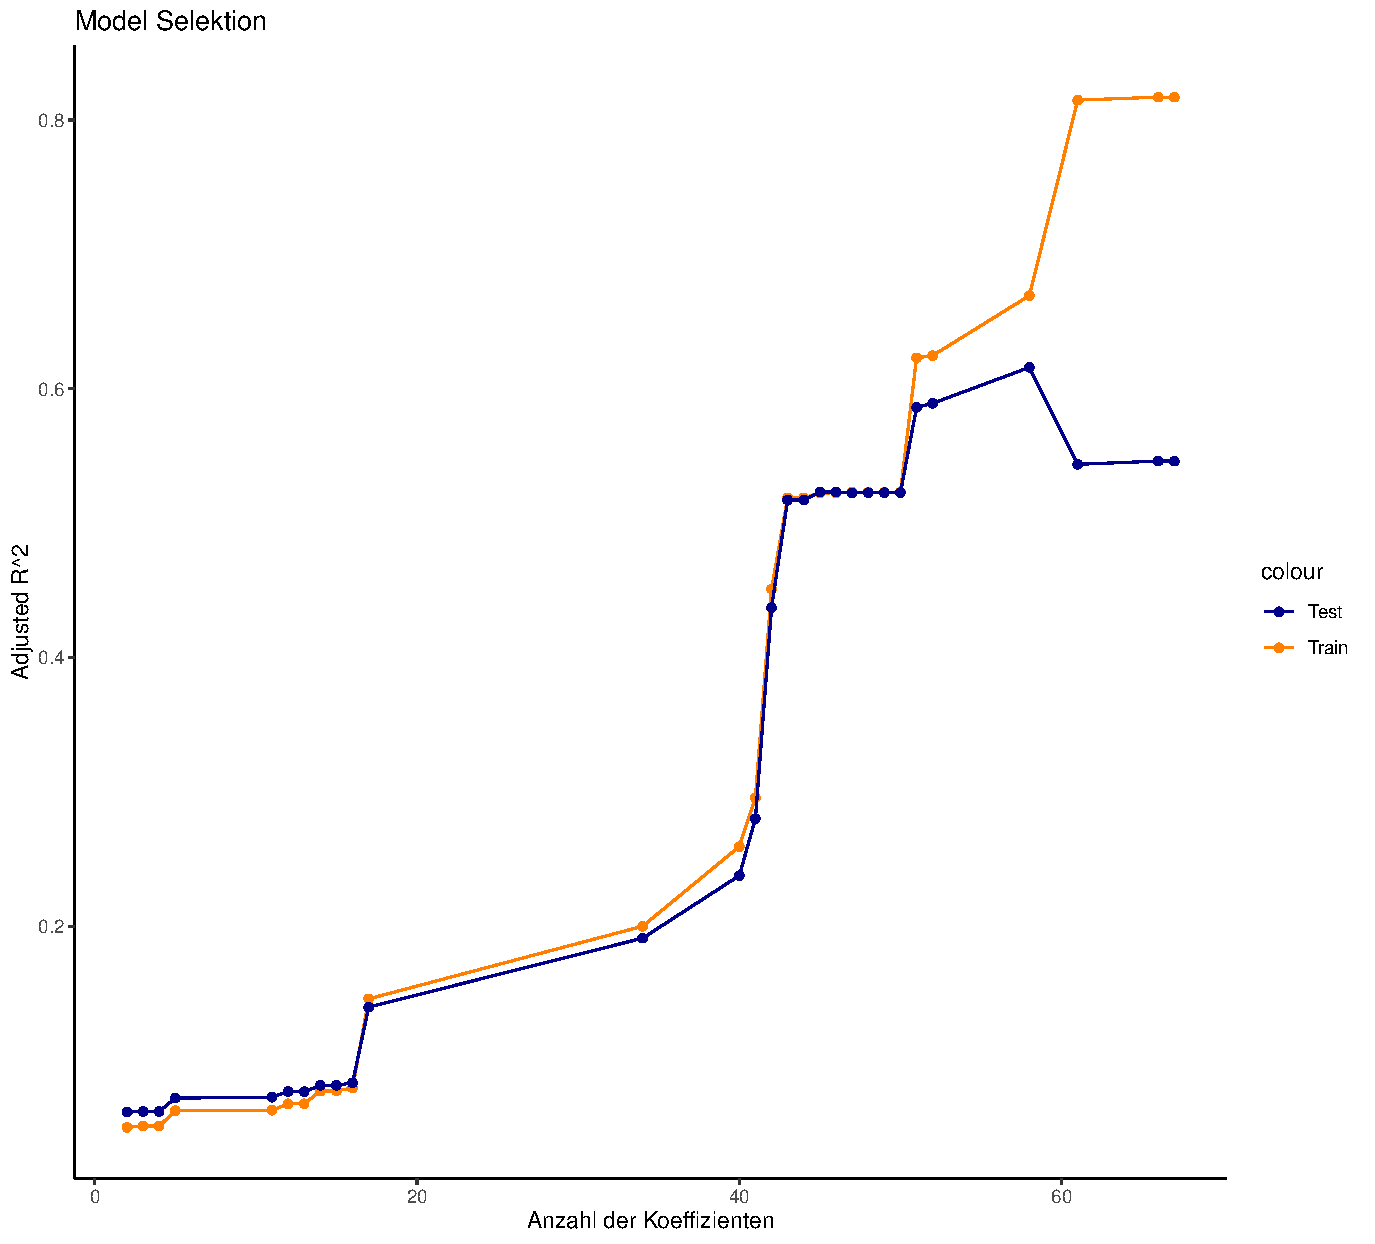
\includegraphics[width=\textwidth]{Plots/ModelSelektion1.pdf}
	\caption{Model Selektion}
	\label{ModelSelektion}
\end{figure}

Auf der Y-Achse der Graphik \ref{ModelSelektion} abgetragen ist die Höhe des Bestimmtheitsmaßes. Auf der X Achse erscheint die Anzahl der Koeffizienten. Mit jedem weiteren Model wurden weitere Variablen hinzugefügt, angefangen mit dem Wetter, Feiertage, Ferien, Zeitliche Variablen, wie das Jahr, Sommer oder Tageszeit bis hin zur geographischen Lage. Wir sehen, dass das Bestimmtheitsmaß, also die Genauigkeit der Vorhersage des Modells, zu nimmt je mehr Variablen hinzufügt werden bis zu einem Punkt, an dem das Bestimmtheitsmaß im Trainingsdatensatz zwar nochmals bedeutend zu nimmt, im Test Datensatz aber abnimmt. Hier geraten wir in das so genannte Overfitting. Das heißt, das Modell, das hier entwickelt wurde, kann zwar die Daten, mit denen es trainiert wurde, extrem gut erklären, sobald wir aber mithilfe des Modells Vorhersagen treffen wollen, auf Grundlage neuer Daten, ist die Genauigkeit der Vorhersagen schlechter, als sie sein dürfte. Das muss verhindert werden. Denn ist ein Modell von Overfitting betroffen, sind in den Variablen Zusammenhänge zu sehen, die sich nicht replizieren lassen.\\
Was löst in unserem Fall das Overfitting aus? Dazu vergleicht man den Regressions Output zweier Modelle in der Tabelle \ref{ZweiModelle}. Das zweite Modell ist jenes, in dem erstmals Overfitting auftritt. Das erste Modell ist das davor, in dem noch kein Overfitting auftritt.

% Table created by stargazer v.5.2.3 by Marek Hlavac, Social Policy Institute. E-mail: marek.hlavac at gmail.com
% Date and time: Sa, Aug 13, 2022 - 12:09:39
	\begin{longtable}{@{\extracolsep{-5pt}}lcc} 
	\caption{Modell Vergleich} 
	\label{ZweiModelle}
	\small 
		\\[-1.8ex]\hline 
		\hline \\[-1.8ex] 
		& \multicolumn{2}{c}{\textit{Dependent variable:}} \\ 
		\cline{2-3} 
		\\[-1.8ex] & \multicolumn{2}{c}{log(Zählstand)} \\ 
		\\[-1.8ex] & (1) & (2)\\ 
		\hline \\[-1.8ex] 
		Temperatur & 0.028$^{***}$ (0.001) & 0.028$^{***}$ (0.001) \\ 
		Temperatur$^2$ & 0.0005$^{***}$ (0.0001) & 0.001$^{***}$ (0.0001) \\ 
		Temperatur$^3$ & $-$0.00002$^{***}$ (0.00000) & $-$0.00003$^{***}$ (0.00000) \\ 
		Leichter Nieselregen & $-$0.198$^{***}$ (0.007) & $-$0.197$^{***}$ (0.006) \\ 
		Starker Nieselregen & $-$0.258$^{***}$ (0.011) & $-$0.260$^{***}$ (0.009) \\ 
		nLeichter Regen & $-$0.334$^{***}$ (0.013) & $-$0.328$^{***}$ (0.010) \\ 
		Moderater Regen & $-$0.369$^{***}$ (0.018) & $-$0.363$^{***}$ (0.015) \\ 
		Starker Regen & $-$0.367$^{***}$ (0.039) & $-$0.354$^{***}$ (0.031) \\ 
		Heftiger Regen & $-$0.199$^{***}$ (0.069) & $-$0.188$^{***}$ (0.056) \\ 
		Wind & $-$0.071$^{***}$ (0.006) & $-$0.074$^{***}$ (0.005) \\ 
		Wind$^2$ & 0.009$^{***}$ (0.001) & 0.009$^{***}$ (0.001) \\ 
		Wind$^3$ & $-$0.001$^{***}$ (0.0001) & $-$0.001$^{***}$ (0.0001) \\ 
		Rel. Feuchte & $-$0.002 (0.002) & $-$0.001 (0.002) \\ 
		Rel. Feuchte$^2$ & $-$0.0001$^{*}$ (0.00003) & $-$0.0001$^{**}$ (0.00003) \\ 
		Rel. Feuchte$^3$ & 0.00000$^{**}$ (0.00000) & 0.00000$^{***}$ (0.00000) \\ 
		Bedeckung & 0.005 (0.006) & 0.0001 (0.005) \\ 
		Bedeckung$^2$ & $-$0.004$^{**}$ (0.002) & $-$0.003$^{*}$ (0.001) \\ 
		Bedeckung$^3$ & 0.0003$^{**}$ (0.0001) & 0.0002$^{*}$ (0.0001) \\ 
		SemesterferienUM & $-$0.131$^{***}$ (0.003) & $-$0.142$^{***}$ (0.003) \\ 
		SchulferienBW & $-$0.154$^{***}$ (0.003) & $-$0.145$^{***}$ (0.003) \\ 
		FeiertagBW & $-$0.398$^{***}$ (0.024) & $-$0.384$^{***}$ (0.020) \\ 
		FeiertagRP & 0.047 (0.151) & 0.068 (0.123) \\ 
		FeiertagBW*RP & $-$0.541$^{***}$ (0.153) & $-$0.573$^{***}$ (0.124) \\ 
		Sommer & 0.050$^{***}$ (0.005) & 0.046$^{***}$ (0.004) \\ 
		Längengrad & 4,275,254.000$^{***}$ (13,711.460) &  \\ 
		Breitengrad & 728,085.000$^{***}$ (2,367.637) &  \\ 
		Längen*Breitengrad & $-$85,858.130$^{***}$ (279.219) &  \\ 
		Längengrad$^3$ & $-$118.352$^{***}$ (1.252) &  \\ 
		K-Adenauer-Brücke &  & 0.877$^{***}$ (0.005) \\ 
		Kurpfalzbrücke &  & 1.555$^{***}$ (0.004) \\ 
		K-Schumacher-Brücke &  & $-$1.982$^{***}$ (0.005) \\ 
		Lindenhofüberführung &  & $-$0.507$^{***}$ (0.005) \\ 
		Neckarauer Übergang &  & $-$0.043$^{***}$ (0.005) \\ 
		Renzstraße &  & 0.869$^{***}$ (0.004) \\ 
		Schlosspark &  & 0.183$^{***}$ (0.005) \\ 
		uniMA\_dist & $-$0.020$^{***}$ (0.0001) &  \\ 
		Corona & 0.008 (0.006) & $-$0.022$^{***}$ (0.005) \\ 
		Kontaktbeschr & $-$0.120$^{***}$ (0.005) & $-$0.120$^{***}$ (0.004) \\ 
		Jahr & 20,824.930$^{***}$ (2,200.256) & $-$3,893.328$^{**}$ (1,788.879) \\ 
		Jahr$^2$ & $-$10.308$^{***}$ (1.090) & 1.941$^{**}$ (0.886) \\ 
		Jahr$^3$ & 0.002$^{***}$ (0.0002) & $-$0.0003$^{**}$ (0.0001) \\ 
		Constant & $-$50,205,702.000$^{***}$  & 2,602,558.000$^{**}$  \\
		 & (1,479,908.000) & (1,203,354.000) \\  
		\hline \\[-1.8ex] 
		Observations & 328,715 & 328,715 \\ 
		R$^{2}$ & 0.672 & 0.784 \\ 
		Adjusted R$^{2}$ & 0.672 & 0.783 \\ 
		\hline 
		\hline \\[-1.8ex] 
		\textit{Note:}  & \multicolumn{2}{r}{$^{*}$p$<$0.1; $^{**}$p$<$0.05; $^{***}$p$<$0.01} \\ 
		\textit{Fixed Effects:}  & \multicolumn{2}{r}{Stunde, Wochentag} \\
\end{longtable}



Beide Modelle unterscheiden sich im Wesentlichen in der Wahl der Fixed Effects. Fixed Effects sind all jene Schätzer, die über die Zeit nicht variieren, also fix sind und nur zwischen den Entitäten variieren (\cite{Stock2003}). In diesem konkreten Fall heißt das, ein Fixed Effect ist eine Variable die zeitlich konstant bleibt, sich aber zwischen den Fahrradzählstationen unterscheidet. Das dient dazu, die Unterschiede zwischen diesen Stationen zu messen und im Modell mit aufzunehmen. Denn fällt der Blick auf die Graphik \ref{BoxplotStationen}, sehen wir, dass die Stationen untereinander recht stark variieren. So herrscht auf der Kurpfalzbrücke, die von der Innenstadt über den Neckar führt, grundsätzlich mehr Radverkehr. Deswegen lässt sich z.B. eine Dummy Variable in das Modell aufnehmen, die eins ist, wenn ein Beobachtungswert von der Kurpfalzbrücke stammte und null ist, wenn der Beobachtungswert von einer anderen Station stammte, dann erklärt diese Variable den Unterschied zwischen der Kurpfalzbrücke und den anderen Stationen im Modell, ohne den ursächlichen Grund dafür zu kennen. Dies erhöht aber die Treffsicherheit (Fit) des Modells, denn nun können die anderen Variablen ihren Einfluss präziser schätzen.\\ 
Eine solche Dummy Variable können wir für sieben von acht Stationen in das Modell aufnehmen. Bei der achten reicht es, wenn alle anderen Dummy Variablen null sind. Andernfalls bekämen wir ein multikollineares Modell, also eines in dem mindestens zwei Variablen linear abhängig von einander sind. Genau auf diese Weise sind wir im zweiten Modell vorgegangen. Dieses beinhaltet eine Dummy Variable für die Kurpfalzbrücke, die Lindenhofüberführung, den Neckarauer Übergang, die Renzstraße und dem Schloßpark/Lindenhof. Die übrige Station an der Kurt Schuhmacher Brücke ergibt sich, wie bereits erklärt, wenn alle anderen sieben Dummy Variablen null sind. Diese Vorgehensweise führt zu einem Bestimmtheitsmaß von 78,3 \%, was sich gut anhört, wie aber bereits gezeigt, größtenteils auf Overfitting zurückzuführen ist.\\
Möglicherweise hängt dies damit zu zusammen, dass die Stations Dummy Variablen zwar Unterschiede erkennen, aber keinen ursächlichen Grund dafür finden. Wenn man aber Lageparameter als Fixed Effekt nutzt, hätte man einen möglichen ursächlichen Grund für den Unterschied, nämlich die Lage. Da Lageparameter zeitlich auch konstant sind, lassen sich diese ebenfalls sehr gut als Fixed Effect nutzen. Deswegen befinden sich im ersten Modell der Längengrad, sowie der quadrierten Längengrad, der Breitengrad, Längen- und Breitengrad miteinander multipliziert (Intersektion) und der Abstand zur Universität Mannheim in \glqq uniMA dist\grqq. Auf den quadrierten Wert des Breitengrades muss verzichtet werden, weil dies wiederum zu Multikollinearität führen würde und im Regressionsoutput ein Fehler auftauchen würde, wie sich zeigte. Auch führt eine Kombination aus Lageparametern und Standort Dummy Variablen zu Fehlern im Regressionsoutput, weswegen wir beide getrennt von einander nutzen.\\
Obwohl das Modell mit den Lageparametern ein kleineres Bestimmtheitsmaß von nur 67,2 \% hat, muss gegen das Modell mit Standort Variablen entschieden werden, wegen einer höheren externen Validität gemessen im Test Datensatz.

\section{Fahrrad Topographie}

Nun steht ein Modell zur Verfügung, dass auf Lagekoordinaten und den Abstand zur Universität Mannheim in Metern zurückgreift, um seine Vorhersagen zu berechnen. Was passiert, wenn wir in dieses Model Lageparameter eingeben, die gar nicht von den Zählstationen selbst stammten sondern von einem beliebigen Straßenpunkt?\\
Dazu kann ein Netz von Koordinaten über die Straßen Mannheims gelegt werden und mit einander so verbunden werden, dass ein Straßennetz erkennbar wird. Allerdings ist das modellierte Straßennetz nicht vollumfänglich, sondern beinhaltet nur eine persönliche Auswahl an Straßen, die meiner persönlichen Ortskenntnis nach, die meiste Relevanz haben. Eine genauere Methode gibt es ohne mehr Daten nicht. Beim Testen des Models fällt auf, dass das Modell, welches im vorherigen Kapitel ausgewählt worden ist, extreme Ausreißer vorhersagt, vergleicht man dies mit der Verteilung des originalen Datensatzes, wie wir in Darstellung \ref{ForecastDistribution} sehen. 

\begin{table}[!htbp] \centering 
	\caption{Verteilung der Vorhersagen} 
	\label{ForecastDistribution} 
	\begin{tabular}{@{\extracolsep{-5pt}}lccccc} 
		\\[-1.8ex]\hline 
		\hline \\[-1.8ex] 
		%\\[-1.8ex] & \multicolumn{8}{c}{log(Zaehlstand)}  \\ 
		\\[-1.8ex] & Min & Median & Mean & Max\\ 
		\hline \\[-1.8ex] 
		Datensatz & 1 & 69 & 116.8 & 955 \\ 
		Vorhersagen von Model 21	 & 19.8 & 150 & 157.6 & 471.3 \\ 
		Vorhersagen von Model 22	 & 19.8 & 149.7 & 157.4 & 470.6 \\ 
		Vorhersagen von Model 23	 & 19.8 & 150.3 & 158 & 472.3 \\ 
		Vorhersagen von Model 24	 & 0 & 374.2 & 63424.4 & 1935375.6\\ 
		Vorhersagen von Model 25	 & 0 & 374.2 & 63424.4 & 1935375.6\\ 
		Vorhersagen von Model 26	 & 0 & 93.4 & 15076.5 & 453753.1\\ 
		Vorhersagen von Model 27	 & 0 & 296.2 & 25163.4 & 593288.3\\ 
		\hline \\[-1.8ex] 
	\end{tabular} 
\end{table} 

Ein Grund für die extremen Ausreißer ist die Einführung der Intersektionsvariabel $Längen*Breitengrad$. Das ist jedoch nicht weiter dramatisch, denn ohne große Verluste bietet sich eines der vorherigen Modelle an, welches in der Übersicht \ref{FinalFinalModel} zu sehen ist. Wendet man genau dieses Modell auf das angelegte Straßennetz Mannheims an, dann kommt man zu der Vorhersage in der Graphik \ref{Topography1}. Zudem ist eine animierte Vorhersage auf YouTube verfügbar (Link: \url{https://youtu.be/EsQ2UK1niJo}). Beiden Darstellungen kann man entnehmen, dass der Verkehr im Westen der Stadt stärker sei, vor allem im Nordwesten. Es gibt jedoch keine Möglichkeiten, diese Aussagen weiter zu prüfen, als durch bloße ungefähre subjektive Ortskenntnis des Verkehrs. Der Nordosten scheint vom Modell überschätzt zu werden.\\
Zudem ist die berechnete Topographie sehr ungenau. Anlaufzentren wie der Bahnhof oder der Jungbusch sollten stärker hervor treten. Außerdem je weiter die Vorhersage vom Stadtzentrum entfernt ist, desto weniger ist sie verlässlich, denn die Beobachtungspunkte, auf denen das Modell zur Vorhersage aufbaut, liegen alle sehr nah am Zentrum. Mit nur acht Beobachtungspunkten auf ein räumliches Model zu schließen, ist zu gewagt, um daraus überzeugende Schlussfolgerungen zu ziehen. Vielmehr dienlich war die Topographie, um zu zeigen, wie weit Overfitting in den Modellen vorhanden war, denn auch wenn Model 24 bis 27 in der Darstellung \ref{ModelSelektion} keinen Hinweis auf Overfitting gaben, zeigte sich in der Anwendung der Modelle außerhalb der geographischen Lageparameter des vorhandenen Datensatzes unrealistische Vorhersagen mit extremen Ausreißern.

% Table created by stargazer v.5.2.3 by Marek Hlavac, Social Policy Institute. E-mail: marek.hlavac at gmail.com
% Date and time: Sa, Aug 13, 2022 - 12:35:28
\begin{table}[!htbp] \centering 
	\caption{Finales Modell: Model 23} 
	\label{FinalFinalModel} 
	\small 
	\begin{tabular}{@{\extracolsep{-15pt}}lc} 
		\\[-1.8ex]\hline 
		\hline \\[-1.8ex] 
		& \multicolumn{1}{c}{\textit{Dependent variable:}} \\ 
		\cline{2-2} 
		\\[-1.8ex] & log(Zählstand) \\ 
		\hline \\[-1.8ex] 
		Temperatur & 0.035$^{***}$ (0.001) \\ 
		Temperatur$^2$ & $-$0.0004$^{***}$ (0.00002) \\ 
		Leichter Nieselregen & $-$0.198$^{***}$ (0.008) \\ 
		Starker Nieselregen & $-$0.254$^{***}$ (0.014) \\ 
		Leichter Regen & $-$0.337$^{***}$ (0.015) \\ 
		Moderater Regen & $-$0.371$^{***}$ (0.022) \\ 
		Starker Regen & $-$0.316$^{***}$ (0.047) \\ 
		Heftiger Regen & $-$0.124 (0.084) \\ 
		Wind & $-$0.034$^{***}$ (0.003) \\ 
		Wind$^2$ & $-$0.001$^{***}$ (0.0004) \\ 
		Rel. Feuchte & $-$0.006$^{***}$ (0.001) \\ 
		Rel. Feuchte$^2$ & 0.00001$^{**}$ (0.00000) \\ 
		Bedeckung & $-$0.002 (0.003) \\ 
		Bedeckung$^2$ & $-$0.001$^{*}$ (0.0003) \\ 
		SemesterferienUM & $-$0.205$^{***}$ (0.004) \\ 
		SchulferienBW & $-$0.066$^{***}$ (0.004) \\ 
		FeiertagBW & $-$0.453$^{***}$ (0.029) \\ 
		FeiertagRP & $-$0.308$^{*}$ (0.184) \\ 
		FeiertagBW*RP & $-$0.137 (0.187) \\ 
		Sommer & 0.043$^{***}$ (0.005) \\ 
		Längengrad & 111.977$^{***}$ (0.297) \\ 
		Breitengrad & 89.465$^{***}$ (0.331) \\ 
		uniMA\_dist & $-$0.001$^{***}$ (0.00001) \\ 
		Corona & $-$0.249$^{***}$ (0.006) \\ 
		Kontaktbeschr & $-$0.087$^{***}$ (0.006) \\ 
		Jahr & 0.032$^{***}$ (0.002) \\ 
		Constant & $-$5,434.835$^{***}$ (19.382) \\ 
		\hline \\[-1.8ex] 
		Observations & 328,715 \\ 
		R$^{2}$ & 0.512 \\ 
		Adjusted R$^{2}$ & 0.512 \\ 
		\hline 
		\hline \\[-1.8ex] 
		\textit{Note:}  & \multicolumn{1}{r}{$^{*}$p$<$0.1; $^{**}$p$<$0.05; $^{***}$p$<$0.01} \\ 
		\textit{Fixed Effects:}  & \multicolumn{1}{r}{Stunde, Wochentag} \\
	\end{tabular} 
\end{table} 

\begin{figure}[!ht]
	\centering
	\includegraphics[width=\textwidth]{Plots/HeatmapFinal1.pdf}
	\caption{Fahrrad Topographie Mannheims an einem vergangenen Tag}
	\label{Topography1}
\end{figure}

\section{Vorhersagevergleich}

Laut der Verwaltung der Stadt Mannheim war die Zählstation an der Renzstraße vom Dezember 2020 bis zum Dezember 2021 defekt. Mittels eines wissenschaftlichen Hochrechnungsverfahren wurden diese fehlenden Daten geschätzt.\\ 
Aufgrund dessen wurden die Daten in diesem Zeitraum von dieser Station aus dem Datensatz ausgelassen, um die Modelle nicht zu verzerren. Ein abschließender Vergleich ist in der Darstellung \ref{Forecast2} zu finden. Die blaue Linie kennzeichnet der Vorhersage des Models dieser Hausarbeit und die rote Linie kennzeichnet die Vorhersage der Hochrechnung.


\begin{figure}[!ht]
	\centering
	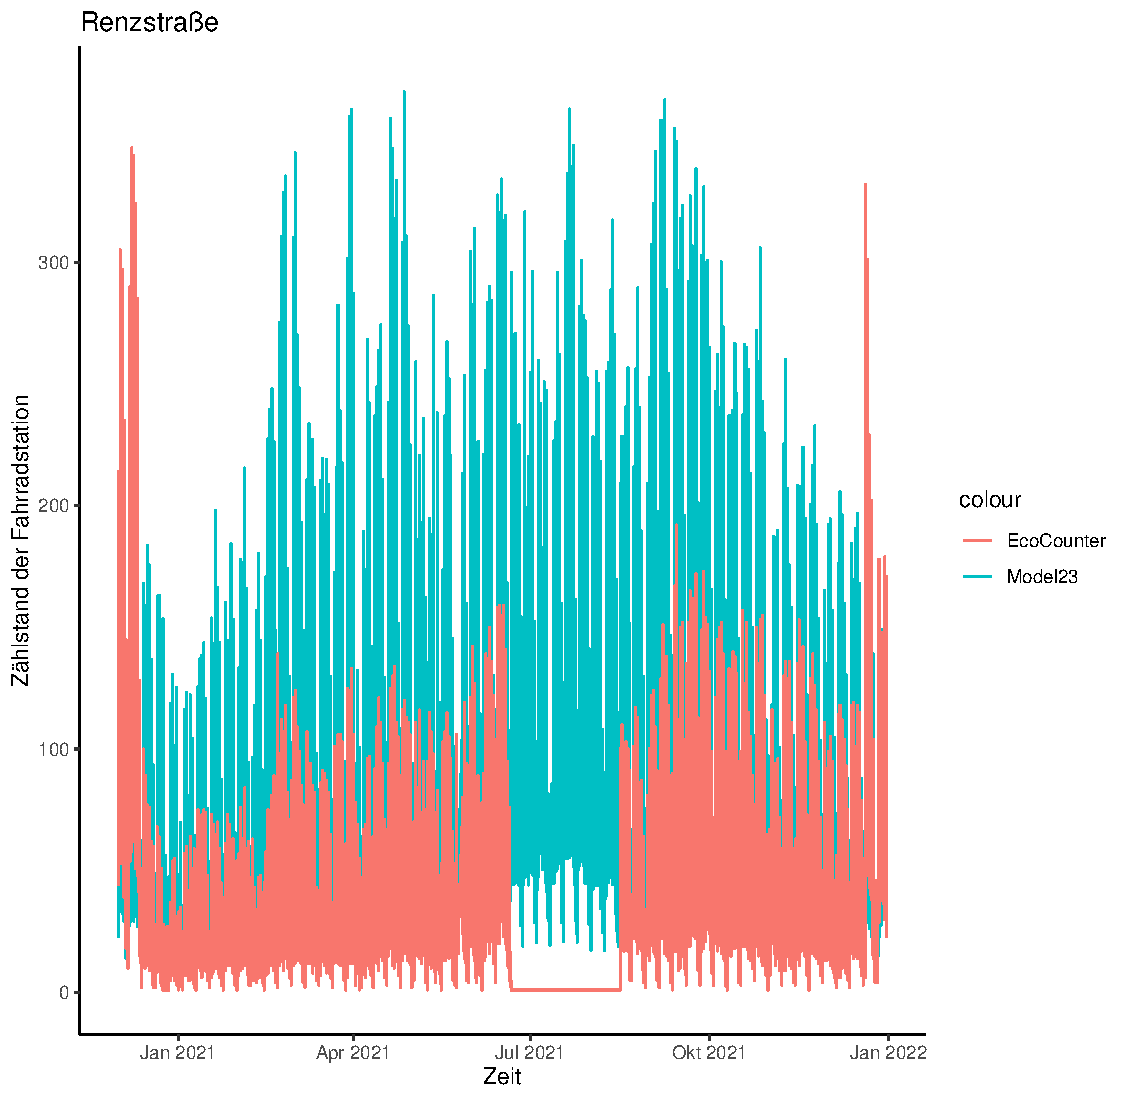
\includegraphics[width=\textwidth]{Plots/Renzstrasse.pdf}
	\caption{Vergleich zur Hochrechnung an der Renzstraße 2021}
	\label{Forecast2}
\end{figure}

\chapter{Fazit}

Diese Hausarbeit bestand im Wesentlichen aus zwei Teilen. Der erste Teil beschäftigte sich mit der Frage, ob auf Grundlage von verschiedenen Parametern das Aufkommen von Fahrradfahrern an den beobachteten Zählstationen erklärt werden kann.\\
Auf der Suche nach Daten, die man nutzen könnte, ließen sich Wetterdaten sowie Daten über Ferien- und Feiertage finden, die ein relativ solides Modell ergaben. Diesem Modell nach sind Niederschlag sowie Ferien- und Feiertage die wichtigsten Variablen bei der Entscheidung Fahrrad zu fahren. Zu erkennen ist auch, dass in Mannheim ein utilitaristischer Verkehr vorherrschend ist.\\
Der zweite Teil versuchte ein Modell zu berechnen, dass nicht nur dazu dienen sollte, beobachtetes Verhalten zu erklären, sondern es auch vorhersagen zu können. Die Frage war, ob sich das Modell extrapolieren lassen könnte, um eine Ansicht der Topographie des Fahrradverkehrs in Mannheim zu erstellen. Dazu mussten 30 verschiedene Modelle berechnet werden. Bei der Auswahl des richtigen Modells fielen Hinweise zum Overfitting einzelner Modelle auf. Weitere Hinweise dazu traten bei der Berechnung der Topographie selbst auf, da dass eigentliche Modell zu extremem Ausreißern führte. Erst durch eine weitere Reduzierung der Koeffizienten entstand eine schlüssige Vorhersage. Auch wenn der Aussagewert der berechneten Topographie angezweifelt werden kann, da keine Daten verfügbar sind, um diese zu prüfen, war dieser Schritt insofern wertvoll, weil durch die Extrapolarisierung weiteres Overfitting der Modelle offen gelegt werden konnte.\\
So zeigt diese Hausarbeit auch, dass durch das Nutzen synthetischer zusätzlicher Datensätze die Robustheit statistischer Modelle erhöht werden kann.\\
Eine robuste Schätzung der Topographie des Fahrradverkehrs könnte möglich sein, wenn mehr geographische relevante Daten in das Modell aufgenommen würden. Interessant wären z.B. auch die Entfernung zum nächst gelegenen Hauptbahnhof oder aber auch zum nächstgelegenen Supermarkt, der Straßentypus auf dem die Zählstation liegt oder die Bevölkerungsdichte. Auch förderlich könnte es sein, diese Analyse auf mehrere Städte auszudehnen und die Ergebnisse in einem Modell zu bündeln.





\chapter{Anhang}

\begin{figure}[!ht]
	\centering
	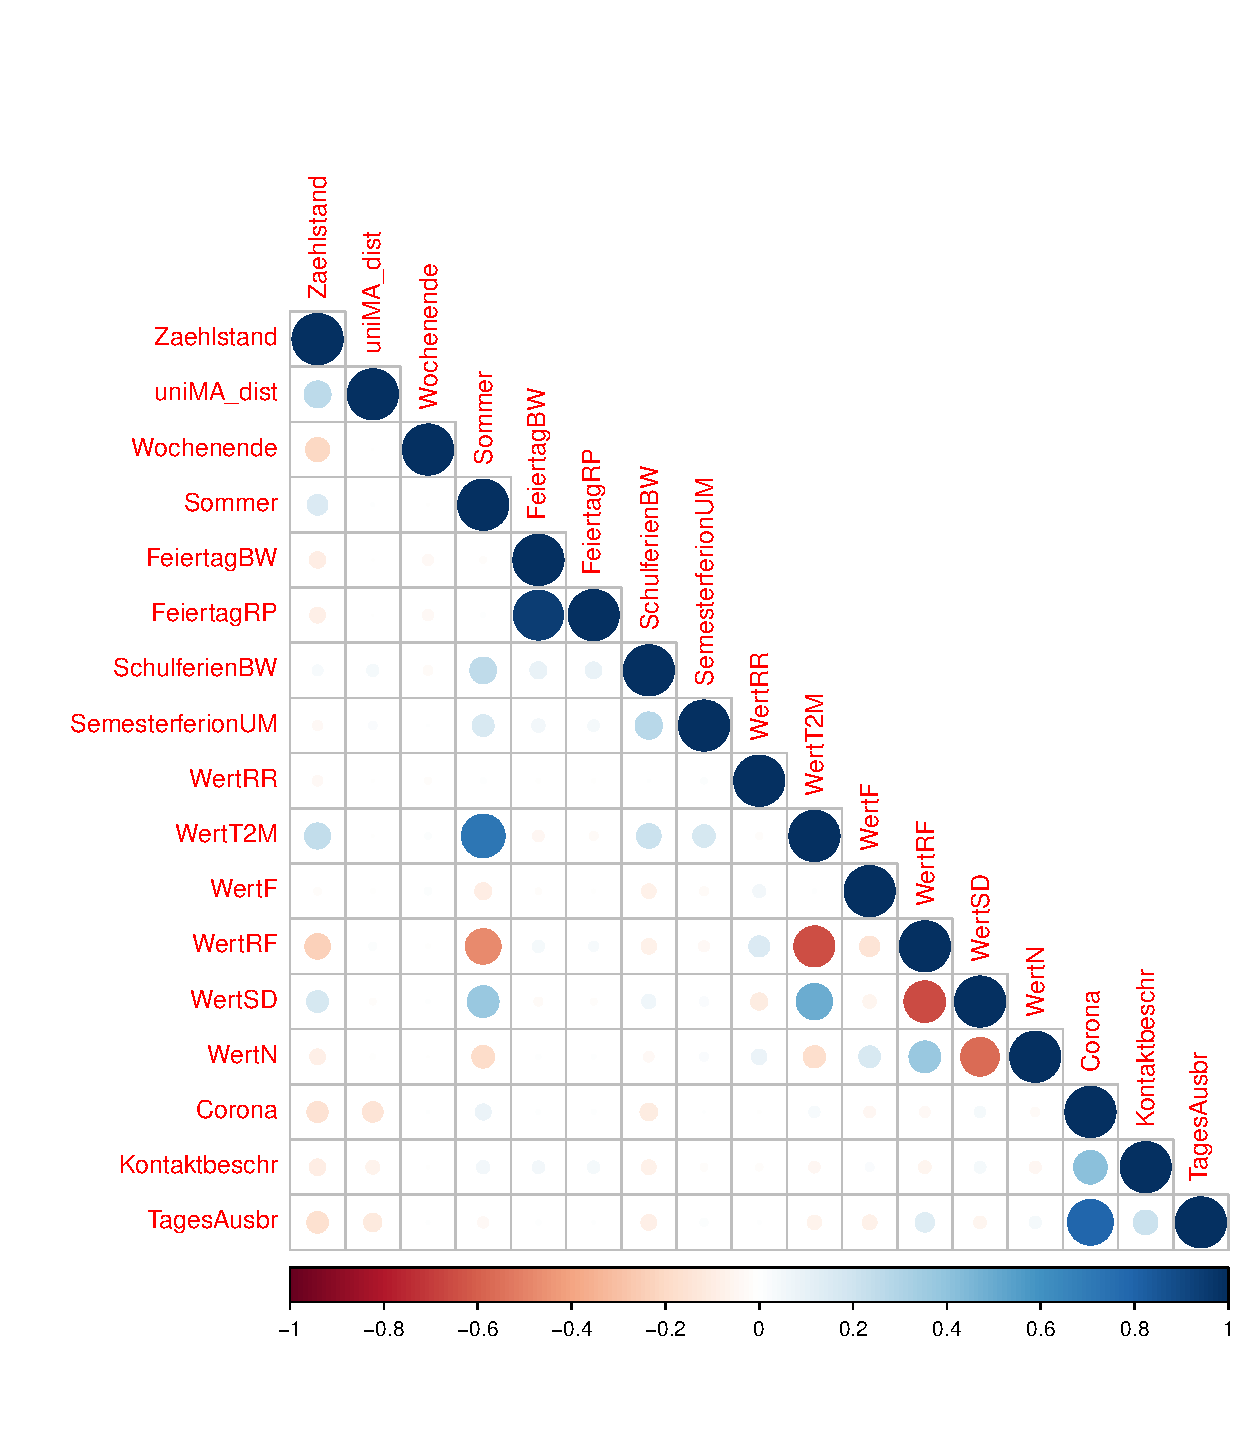
\includegraphics[width=\textwidth]{Plots/Corr_Plot.pdf}
	\caption{Korrelations Plot 
	}
	\label{Figure3}
\end{figure}

\begin{figure}[!ht]
	\centering
	\includegraphics[width=\textwidth]{Plots/Monatliche_Temperatur_Niederschläge.png}
	\captionsource{Monatliche Durchschnittliche Temperaturen und maximale Niederschläge nach Tageszeiten 2018}{
		DWD, eigene Darstellung
	}
	\label{Figure4}
\end{figure}

\begin{figure}[!ht]
	\centering
	\includegraphics[width=\textwidth]{Plots/Taegliche_Temperatur_Niederschläge.png}
	\captionsource{Tägliche Durchschnitts Temperaturen und monatliche maximale Niederschläge nach Tageszeiten 2018}{
		DWD, eigene Darstellung
	}
	\label{Figure5}
\end{figure}






\begin{table}[!htbp] \centering 
	\caption{Wetterdaten als täglichen Niederschlag und Höchsttemperatur} 
	\label{ExtraWetter} 
	\begin{tabular}{@{\extracolsep{-5pt}}lccccc} 
		\\[-1.8ex]\hline 
		\hline \\[-1.8ex] 
		%\\[-1.8ex] & \multicolumn{8}{c}{log(Zaehlstand)}  \\ 
		\\[-1.8ex] & Standardmodell & & & taeglWetter & \\ 
		\hline \\[-1.8ex] 
		
		Leichter Nieselregen & -0.183609$^{***}$ & (0.015146) &  &  & \\ 
		
		Starker Nieselregen & -0.248702$^{***}$ & (0.012068) &  &  & \\ 
		
		Leichter Regen & -0.331162$^{***}$ & (0.020894) &  &  & \\ 
		
		Moderater Regen & -0.353010$^{***}$ & (0.018780) &  &  & \\ 
		
		Starker Regen & -0.373162$^{***}$ & (0.043303) &  &  & \\ 
		
		Heftiger Regen & -0.208576$^{**}$ & (0.051431) &  &  & \\ 
		
		Täglicher Regen &  &  &  & -0.001410$^{***}$ & (0.000094)\\ 
		
		Temperatur & 0.036044$^{***}$ & (0.004718) & & \\ 
		
		Temperatur$^2$ & -0.000482$^{***}$ & (0.000052) &  &  & \\ 
		
		TagesHöcshttemp & &  &  & 0.034072$^{***}$ & (0.005517)\\ 
		
		TagesHöcshttemp$^2$ &  &  &  & -0.000353$^{**}$ & (0.000081)\\ 
		
		Wind & -0.040923$^{***}$ & (0.002549) & $<$ & -0.035015$^{***}$ & (0.002136)\\ 
		
		rel. Feuchte & -0.003787$^{**}$ & (0.001078) & $>$ & -0.004337$^{**}$ & (0.000948)\\ 
		
		Sonne & -0.000118 & (0.000086) & $>$ & 0.000179 & (0.000115)\\ 
		
		Bedeckung & -0.008657$^{***}$ & (0.001074) & $<$ & -0.000208 & (0.000694)\\ 
		
		FeiertagBW & -0.459770$^{***}$ & (0.080732) & $<$ & -0.444115$^{**}$ & (0.085660)\\ 
		
		FeiertagRP & -0.414345$^{***}$ & (0.059184) & $>$ & -0.427126$^{***}$ & (0.065291)\\ 
		
		SchulferienBW & -0.138772$^{***}$ & (0.020264) & $<$ & -0.138865$^{***}$ & (0.020478)\\ 
		
		SemesterferienUM & -0.159223$^{**}$ & (0.030637) & $<$ & -0.150810$^{**}$ & (0.036192)\\ 
		
		Sommer & 0.082386$^{**}$ & (0.020602) & $>$ & 0.072395$^{*}$ & (0.022105)\\ 
		
		Kontaktbeschr & -0.133188$^{**}$ & (0.026552) & $>$ & -0.139072$^{**}$ & (0.026333)\\ 
		
		Observations & 410,891 & & & 410,891 & \\ 
		Adjusted R$^{2}$ & 0.817542 & & & 0.817554 & \\  
		\hline \\[-1.8ex] 
		\textit{Fixed Effects:} & \multicolumn{5}{l}{Standort: 8;Stunde: 18;Wochentag: 7;Jahr: 9} \\ 
		\textit{Notes:} & \multicolumn{5}{l}{$^{***}$Significant at the 1 percent level.} \\ 
		& \multicolumn{5}{l}{$^{**}$Significant at the 5 percent level.} \\ 
		& \multicolumn{5}{l}{$^{*}$Significant at the 10 percent level.} \\ 
	\end{tabular} 
\end{table} 

\begin{table}[!htbp] \centering 
	\caption{Beispielhafte Vorhersagen} 
	\label{ForecastsExample} 
	\begin{tabular}{@{\extracolsep{-5pt}}lccccc} 
		\\[-1.8ex]\hline 
		\hline \\[-1.8ex] 
		%\\[-1.8ex] & \multicolumn{8}{c}{log(Zaehlstand)}  \\ 
		Beobachtungen: & (1) & (2) & (3) \\ 
		\hline \\[-1.8ex] 
		Temperatur & 28°C & 4°C & 12°C\\
		Niederschlag & 0 mm & 3 mm &  3 mm\\
		Bedeckungsgrad & 1/8 & 2/8 & 8/8\\
		Windgeschwindigkeit &  1 m/s & 3 m/s & 4 m/s\\
		Luftfeuchtigkeit &  75 \% & 85 \% & 71 \% \\
		Sonne & 19.22 & 19.22 & 19.22\\
		Feiertag BW & Nein & Ja & Nein \\
		Feiertag RP & Nein & Ja & Nein \\
		Schulferien BW & Nein & Ja & Nein \\
		Semesterferien & Ja & Nein & Nein \\
		Uhrzeit & 16:00 & 11:00 & 15:00 \\
		Wochentag & Sonntag & Freitag & Mittwoch \\
		Monat & August & November & Juni \\
		Jahr & 2018 & 2018 & 2018 \\
		Kontakteinschr & Nein & Nein & Nein \\
		\hline \\[-1.8ex]
		Vorhersagen: & 361 & 31 & 161 \\ 
		\hline \\[-1.8ex] 
	\end{tabular} 
\end{table} 

\begin{figure}[!ht]
	\centering
	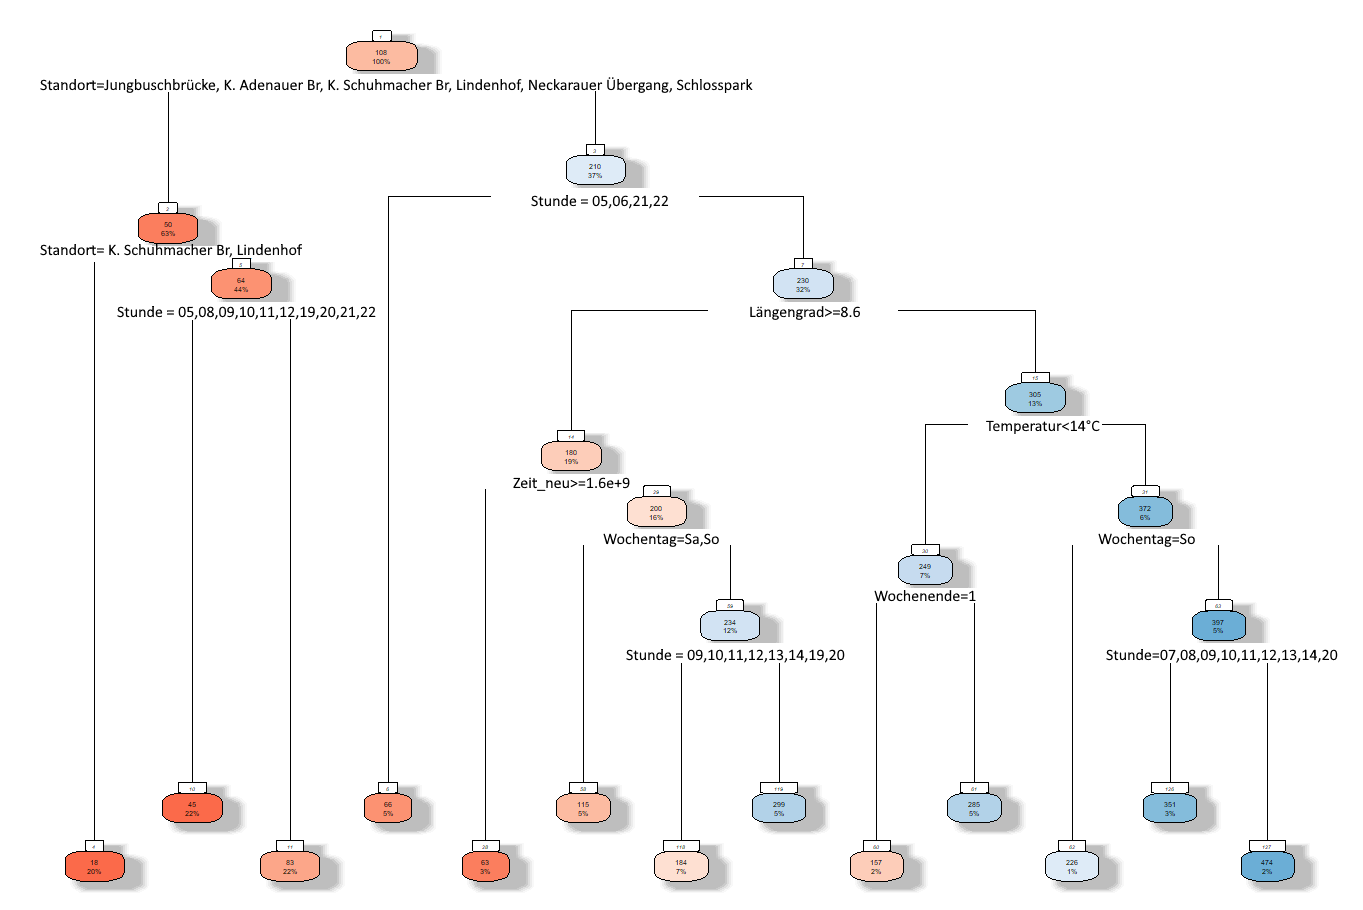
\includegraphics[width=\textwidth]{Plots/Entscheidungsbaum.png}
	\caption{Entscheidungsbaum}
	\label{DecisionTree}
\end{figure}

\newpage
\addcontentsline{toc}{chapter}{Literaturverzeichnis}
\bibliography{bib1}

\end{document}

